\documentclass[12pt]{iopart}
% \usepackage[numbers,sort,compress]{natbib}
\usepackage{iopams}  
\usepackage[utf8]{inputenc}
\usepackage{graphicx}
\usepackage{dcolumn}
\usepackage{bm}
\usepackage{enumitem}
\usepackage{siunitx}
\usepackage{booktabs}
\usepackage{hyperref}
\hypersetup{
    colorlinks=true,
    linkcolor=blue,
    filecolor=magenta,      
    urlcolor=cyan
    }
\usepackage{amsfonts}
\usepackage{nicefrac}
\usepackage{microtype}
\usepackage{lipsum}
\usepackage{multirow}
\usepackage{color}
\usepackage{lineno}
\usepackage[normalem]{ulem}
\usepackage{placeins}
\usepackage{xspace}
\usepackage{soul}

\usepackage{geometry}
\geometry{left=2cm, right=2cm, bottom=1.5cm}
\linespread{1.5}

\renewcommand*\abstractname{Summary}
\newcommand{\NA}{\ensuremath{\text{---}}\xspace}
\newcommand{\PH}{\ensuremath{\mathrm{H}}\xspace}
\newcommand{\kt}{\ensuremath{k_{\mathrm{T}}}\xspace}
\newcommand{\ptmomentum}{\ensuremath{p_{\mathrm{T}}}\xspace}
\newcommand{\GeV}{\ensuremath{\,\text{Ge\hspace{-.08em}V}}\xspace}
\newcommand{\TeV}{\ensuremath{\,\text{Te\hspace{-.08em}V}}\xspace}
\newcommand{\hlsfml}{\texttt{hls4ml}\xspace}

\makeatletter
\def\@maketitle{%
  \newpage
  % original definition of \@maketitle minus the \newpage or \clearpage command
}


\begin{document}
\title[Real-time AI for HL-LHC and beyond (SNSF SG Proposal, T. K. \AA rrestad)]{
\underline{SNSF Starting Grant Proposal:}\\\vspace{5mm}
% {New Physics detection with unsupervised AI}}
{Detecting New Physics at 40 MHz:\\
Enhancing the CMS hardware event filtering system with real-time AI for High Luminosity LHC and beyond}}
\author{Thea Kl\ae boe \AA rrestad}
\address{ETH Zürich, Switzerland}
 \ead{thea.aarrestad@cern.ch}
\date{\today}



\begin{abstract}
Despite being our current best description of nature, we know that The Standard Model of particle physics breaks down at short distances. It is an effective field theory, to be replaced by something more fundamental at shorter distance scales. Nevertheless, searches for new physics beyond the standard model at the CERN Large Hadron Collider (LHC) have thus far been futile. The reasons for this may be that a) the cross section of the signal is too small and more data is needed, or b) that we are not sensitive to it using our currents methods of detection. This project will address both of these using state-of-the art Machine Learning. The LHC will undergo substantial upgrades to its High-Luminosity phase (HL-LHC), with construction work beginning in 2026 and first collisions taking place in 2029~\cite{LHC2022LongTerm}. This upgrade will result in a factor of ten times more data delivered to the CMS experiment, allowing for the measurement of extremely rare processes. Nevertheless, this increase in accumulated data comes at the cost of data complexity: the number of concurrent proton-proton collisions will increase from the present 60 to as many as 200 in the HL-LHC phase.

The ultimate limiting factor for many searches for New Physics with the CMS experiment is the Level-1 hardware trigger. Here, it is decided which of the 40 million proton-proton collision events occurring every second are to be stored for further processing, and which are to be discarded and hence are lost forever. Over 98 \% of all collision events are rejected at this stage so high selection accuracy is crucial for physics analyses. Due to the extreme increase in data complexity, the Level-1 trigger will be completely redesigned for HL-LHC in order to cope with a data rate of 63 Tb/s, corresponding to 5\% of the total internet traffic, within a latency of 12~$\mu$s~\cite{tdr}. This is ten orders of magnitude more data than the current LHC Level-1 trigger receives, with only a factor of 3 more time to process the data. Much of the data comes from the inclusion of information from the CMS tracker, offering a highly precise measurement of charged particle momentum, as well as more granular detectors. The inclusion of this information will result in an unprecedented resolution at Level-1; after 12~$\mu$s we will have the same level of detail of information of every single event as we would only have offline only for a small subset of the data. 
The growing complexity and volume of data necessitate algorithms capable of swiftly and accurately processing high-dimensional information. This requirement has driven substantial research into machine learning-based algorithms, which have achieved a high level of success~\cite{tdr}.
This work will become increasingly important in the years leading up to the start of data taking at the HL-LHC and will also be of significant importance for future experiments at the new Future Circular Collider.
Besides ensuring that data resolution and physics quality are upheld to enable analyses with the same level of sensitivity as the current LHC, the HL-LHC era will be a time dedicated to exhaustive exploration in the search for New Physics, leaving no stone unturned.
Despite conducting hundreds of searches for a wide variety of potential new particles, none have been discovered to date. However, there remain unexplored areas within the data where a signal might be detected. Addressing this will necessitate a transformation in our approach to conducting these searches.

In this proposal, I suggest two complementary projects aimed at addressing points a) and b) and the challenges listed above. These projects are designed to enhance the sensitivity of the CMS to new physics phenomena. The first project involves fundamentally changing the process of event reconstruction and selection in the Level-1 trigger. Taking advantage of techniques from natural language processing, leveraging models trained unsupervised on vast amounts of data, we will move towards end-to-end ML-based reconstruction. The aim is to simultaneously improve accuracy and processing time, and work developed here would apply to both the HL-LHC and future colliders. The approach uses ultra-fast ML algorithms executed on field programmable gate arrays (FPGAs). This builds on the pioneering work currently being undertaken by my group at ETH. The techniques developed for this project have the potential to be applied not only in particle physics, but also in data processing for large telescope arrays and neutrino experiments. The second project focuses on the development of a real-time, signal-independent discovery analysis. This analysis would have the capability to analyze every single collision within CMS, bypassing the Level-1 trigger by running in separate system. Utilizing open world learning, where an agent starts with a set of known classes and then detects and learns new ones over time from a non-stationary stream of data, the objective is to discover a wide array of potential new physics signatures in a manner that is not specific to any one signal.
This approach will help us maximize the utilization of the HL-LHC data collection period by ensuring that we do not overlook potential evidence of new physics simply because our search is concentrated in the wrong place.
\end{abstract}

\makeatother

\section{Section a: State-of-the-art and objectives}

At the CERN Large Hadron Collider (LHC), bunches of trillions of protons are brought to collide in the center of the four particle detectors around the LHC ring: ATLAS, CMS, ALICE and LHCb~\cite{LyndonEvans_2008}. This generates showers of new outgoing particles that produce signals in the particle detectors located around the interaction point. Due to the high frequency of collisions, every 25 ns, and large number of read-out channels, $\mathcal{O}(10)$~million, an enormous amount of data is generated. For the CMS experiment, this is $\mathcal{O}(100)$~Tb/s. These signals are read out using custom electronics mounted on support structures inside the detectors. This large data rate can not be read out and stored as it would require a significant amount of electronics and power supply inside the detector, obstructing the path of generated particles and reducing the detector sensitivity. Rather, the data rate is reduced by a two-stage filtering system, the trigger. While data is buffered inside the detector on detector front-end electronics, a subset of the detector information is sent through high speed optical links to a radiation-shielded cavern located next to the detector. Here, the first stage of the event filtering system, the Level-1 trigger (L1T), is responsible for reducing the data rate by two orders of magnitude within the buffering time of $\mathcal{O}(1)\mu s$. Due to the strict latency constraints, this processing is done fully in firmware on $\mathcal{O}(1000)$~field programmable gate arrays (FPGAs). The complexity of the data requires hundreds of reconstruction algorithms to run in parallel on several collision events simultaneously, which requires each algorithm to use minimal resources and time. The extreme latency and bandwidth requirements for the L1T system is unique and requires novel solutions in terms of IO and algorithms. Due to their ability to efficiently and accurately process and parameterize high dimensional input, Machine Learning (ML) algorithms are increasingly being explored as faster and better replacements of the classical algorithms currently in use in the L1T. The extremely low latency and resource requirements for ML algorithms deployed in the L1T system has led to the development of dedicated software libraries that facilitates the training and translation of ML models into efficient FPGA firmware; hls4ml~\cite{hls4ml,qkerashls4ml,Aarrestad_2021,Ghielmetti_2022} for deep neural networks and Conifer~\cite{Summers_2020} for decision trees, work I have been an integral part of for the past five years. This has allowed for the first deep neural networks to be integrated into the L1T system, work done during the first two years of my SNSF Ambizione grant, running inference within a few tens of nanoseconds~\cite{CMS-DP-2023-079} and expected to collect data for offline analysis in 2024.

\subsection{HL-LHC and beyond: Future Challenges}
With the rapid development of hls4ml and Conifer, deep neural network and decision tree sub-microsecond inference in L1T systems is a reality. However, there are significant challenges ahead. In order to study increasingly rare physics processes in the LHC detectors, the LHC will be upgraded to its High Luminosity phase (HL-LHC), allowing the experiments to collect a factor of ten more data~\cite{tdr}. On the other hand, this involves a significant trade-off: The number of simultaneous proton collisions will triple, leading to an increased event complexity. To cope with this, more granular detectors will be installed, demanding even more complex reconstruction algorithms due to the large increase in read-out channels. For the first time, the CMS L1T will also receive information from the inner tracking system. This will require the reconstruction of hundreds of charged particle tracks from thousands of detector hits, within a maximum latency of $5\mu s$. The input data rate to the L1T systems will increase by one order of magnitude, corresponding to around 5\% of the total internet traffic~\cite{tdr}. This necessitates the design and implementation of significantly more advanced ML algorithms for the reconstruction, correction and selection of proton collision events~\cite{Elabd2022GNNFPGAs,Brown2023NNPrimaryVertex,Iiyama2021DistanceWeightedGNN,Que2022OptimizingGNN,CMS2022NNAlgorithm,CMS2023ElectronReconstruction,CMS2023ContinualLearning}.

Having access to charged particle tracks and more granular information, will result in unprecedented resolution in the Level-1 system. This enhanced resolution is achieved by using these tracks in conjunction with data from the calorimeters and muon chambers. The process of assembling particles and delineating their paths through the detector is known as \textit{Particle Flow (PF)}~\cite{Sirunyan_2017}. For the first time, this method, which is the most powerful event reconstruction technique used in offline processing, will be implemented on FPGAs within the Level-1 trigger. The expected improvement from running these algorithms in the trigger is shown in Figure~\ref{fig:phase2_physics}. In order to select interesting events, one usually defines thresholds on certain physical quantities where every event which passes one or more thresholds is kept for further offline analysis. Lowering this threshold results in increased signal efficiency, for instance for potential New Physics processes, but will also lead to decreased signal purity, collecting more events deemed uninteresting.

Figure~\ref{fig:phase2_physics} shows the distribution of two key variables used in selecting events in the Level-1 trigger, for three different interesting physics processes. Events positioned to the right of the vertical lines are retained for further offline analysis, while the ones that fall on the left are discarded by the Level-1 trigger. The inclusion of tracks and PF (represented by the solid line) markedly enhances signal acceptance compared to the present default method (indicated by the dashed line), thereby improving the sensitivity in the search for these processes.
\begin{figure}[h]
  \centering
  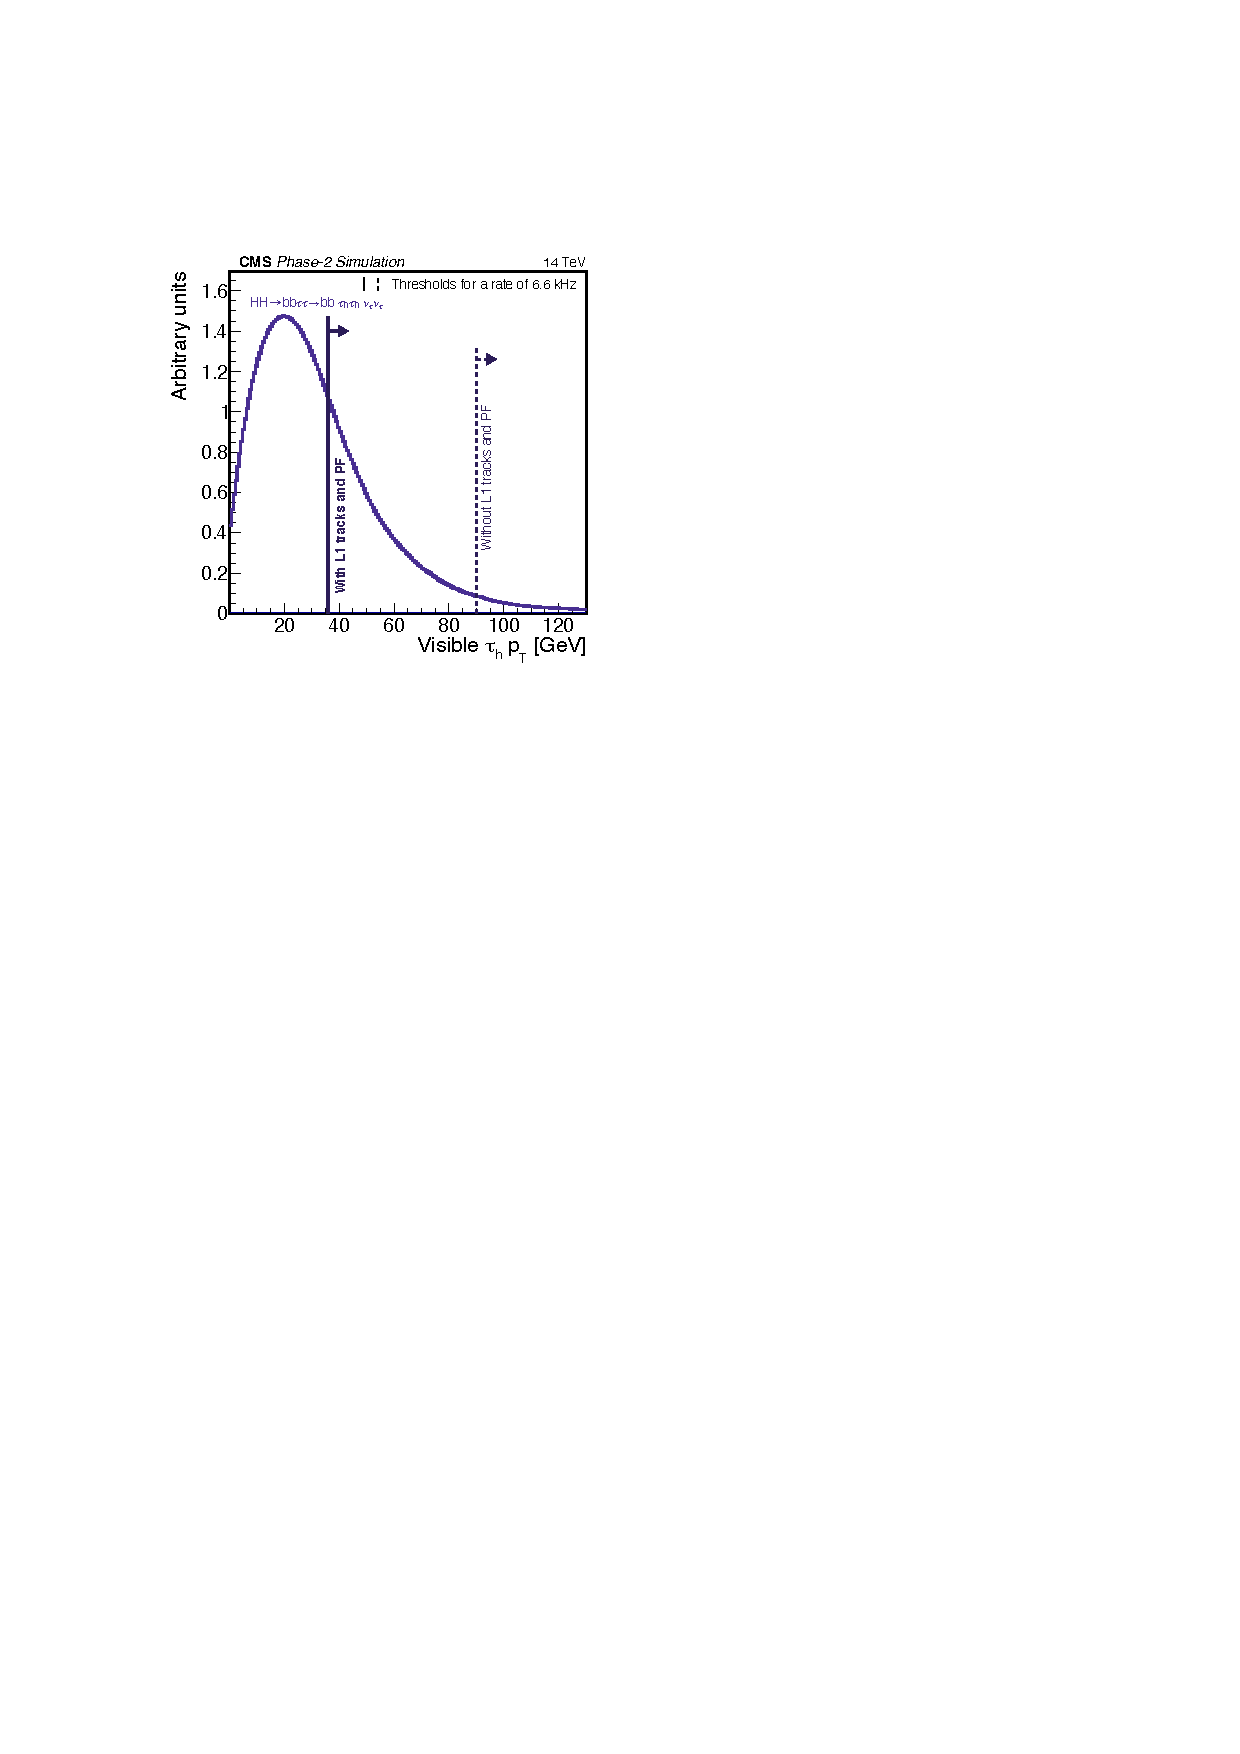
\includegraphics[width=0.49\textwidth]{figures/phase2_tauh.pdf}
  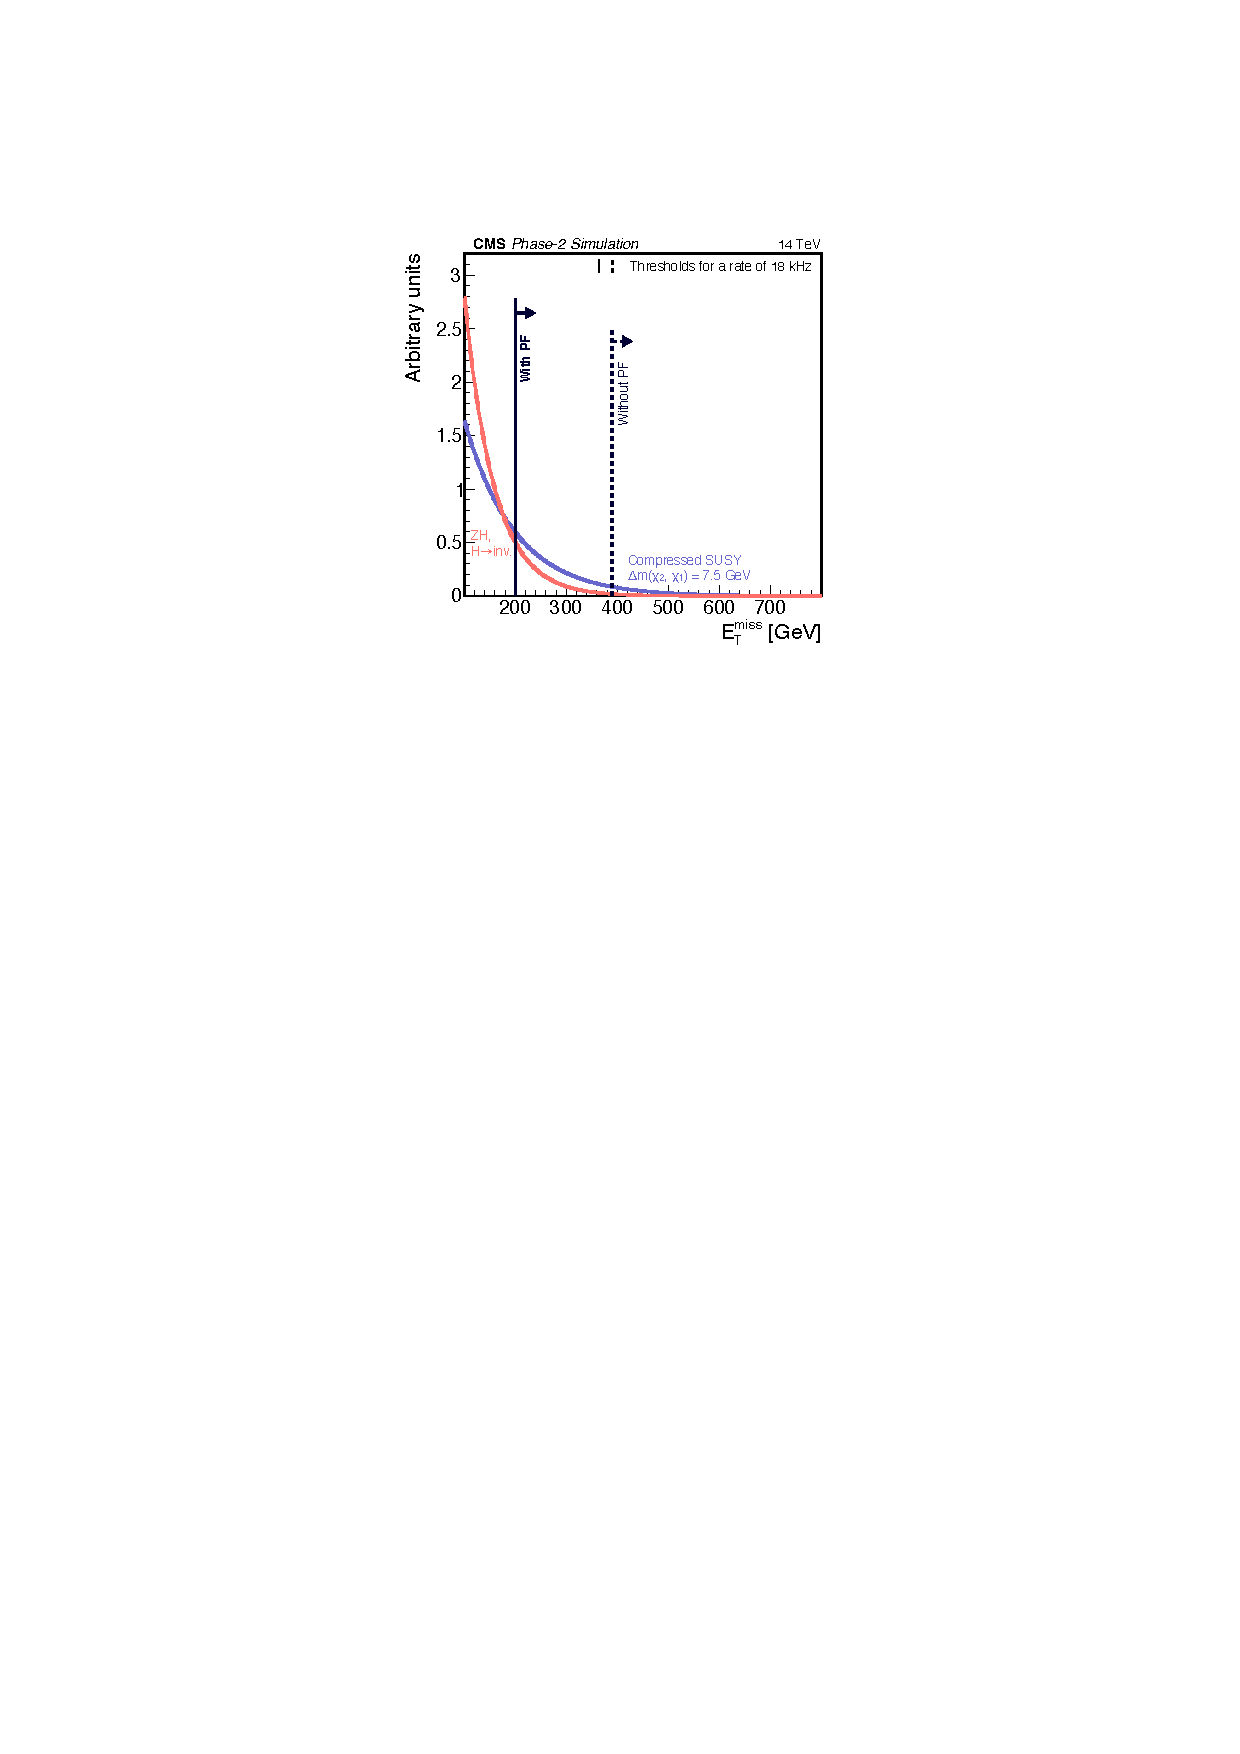
\includegraphics[width=0.49\textwidth]{figures/phase2_etmiss.pdf}
  \caption{The inclusion of charged particle tracks~\cite{tdr}.} % Caption
  \label{fig:phase2_physics} % Label for referencing
\end{figure}
In addition to enhancing signal acceptance, the availability of such high resolution for the first time opens up the possibility of conducting an analysis of data reconstructed at Level-1. This provides the unique opportunity to access information on every single collision occurring inside CMS, though at a slightly lower resolution than what is achievable offline. However, the challenge lies in the limited buffering time of $12\mu s$, rendering any attempt at such detailed analysis impractical.

Due to this, CMS will deploy a novel parasitic system that acquires the L1 trigger data at the full bunch crossing rate of 40 MHz and analyzes certain interesting topologies at the full rate~\cite{40MhzSc}, referred to as \textit{40 MHz scouting}. In this system one can either perform a real-time analysis of the L1 data and/or store a subset of the events in a compact format. This system will run in parallel to the Level-1 trigger and is the only place one will have access to the full CMS collision data, bypassing any trigger selection. This system will offer access to physics signatures that would evade the typical Level-1 to Offline chain, for instance signatures which have to large irreducible backgrounds (for instance narrow resonances of unknown mass) or cases where the signal identification itself requires an algorithm that cannot fit within the Level-1 fixed latency.
A sketch of this system is shown in Figure~\ref{fig:scouting}.
\begin{figure*}[htb!]
    \centering
    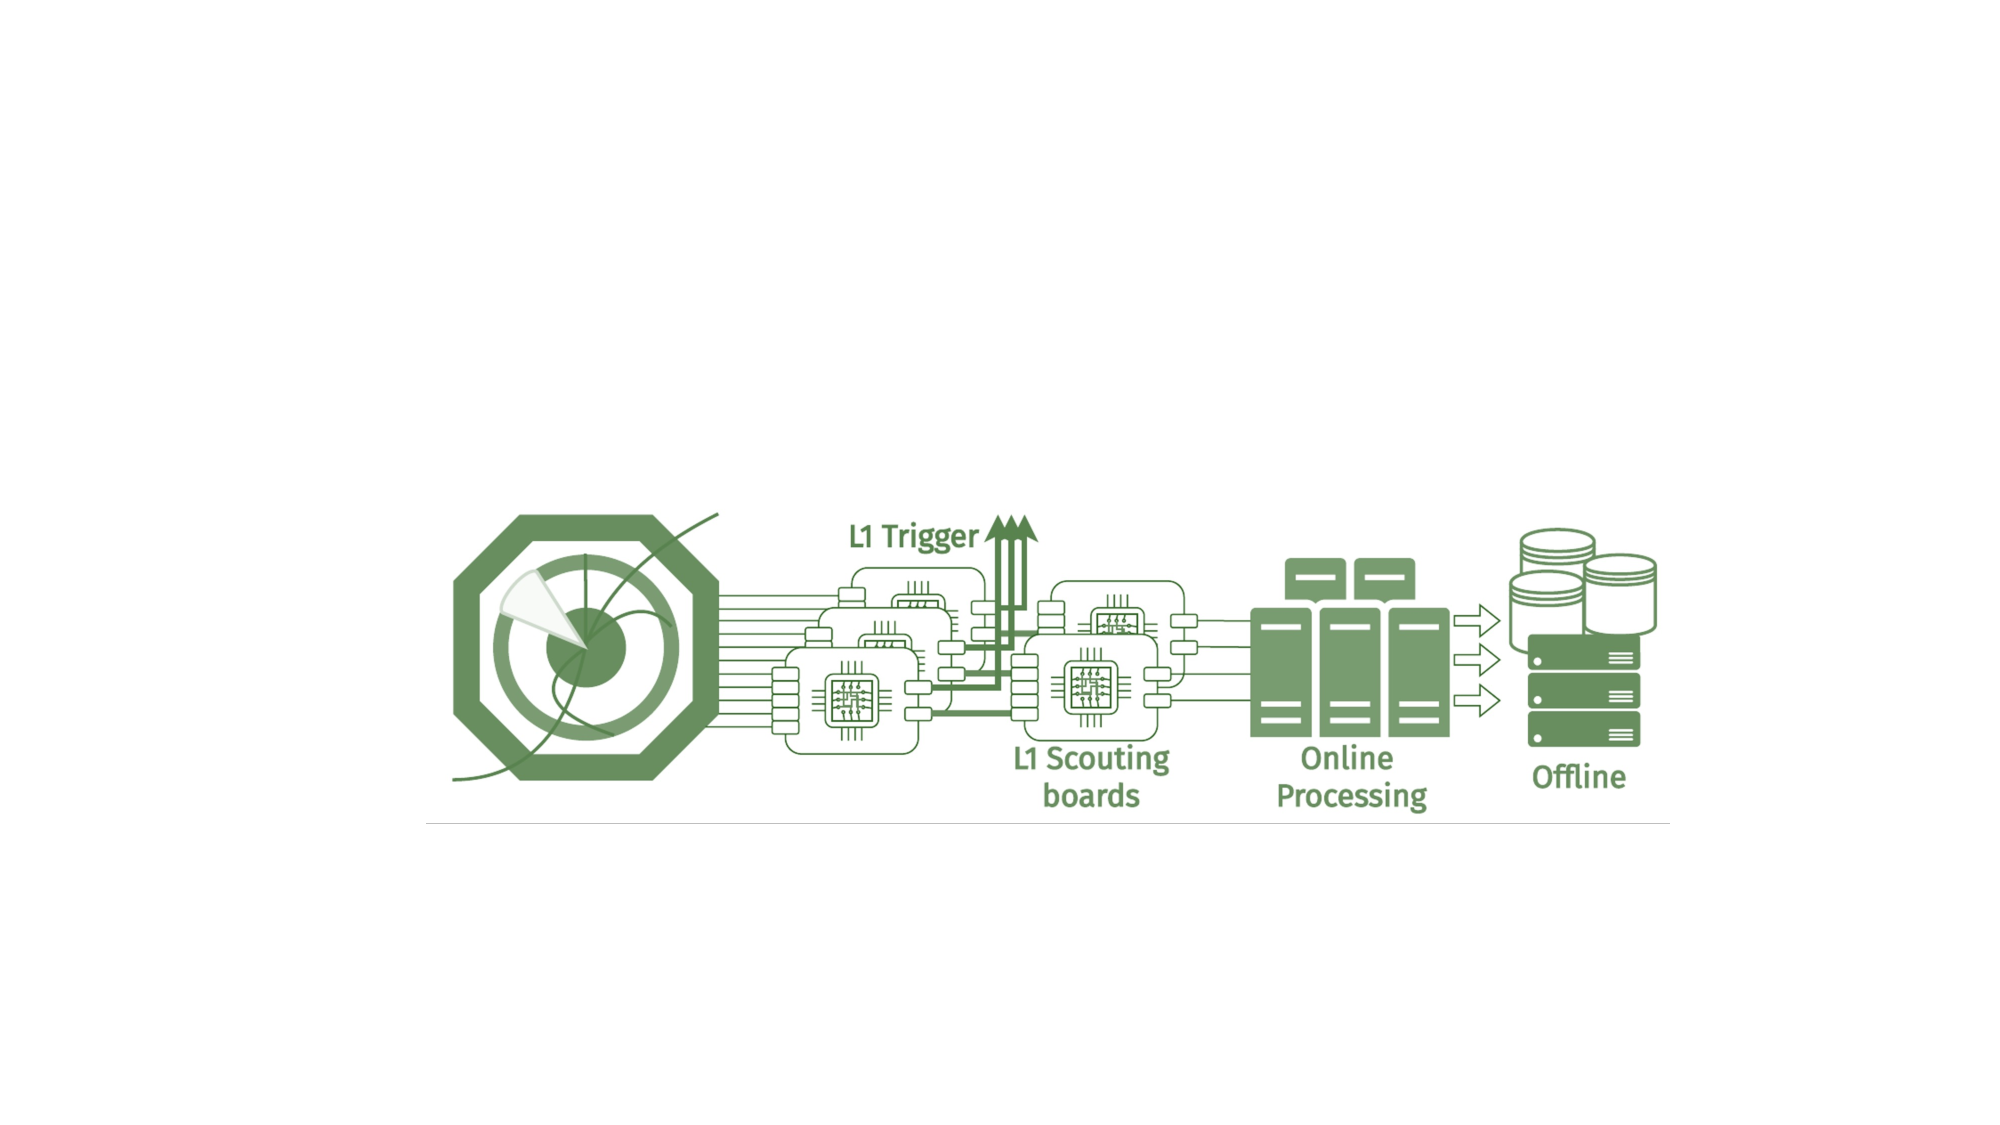
\includegraphics[width=0.99\textwidth]{figures/40mhz_scout.pdf}
    \caption{A sketch of the 40 MHz scouting system prototype planned for HL-LHC, which includes calorimeter- and muon-scouting. The system consists of a parallel readout chain which processes copies of the output streams feeding the Level-1 components. It consists of optical links connected to the L1 triggers, an input board consisting of FPGAs performing local pre-processing, zero-suppression and short-time buffering. This then feeds into other accelerators (GPUs, CPUs) that use distributed algorithms to extract features. Finally, the data goes into a distributed global stream processing system and is stored in a feature database~\cite{tdr}.
    }
    \label{fig:scouting}
\end{figure*}

\subsection{Model-independent searches for New Physics}
An important limiting factor in the search for New Physics is related to how such searches are designed. Typically, a specific New Physics model is assumed and a hypothesis test based on whether the assumed signal is present in the data or not is performed. Such a search is model-dependent and requires one to assume a given signal scenario before the search is conducted. However, there's a growing likelihood, evidenced by the absence of NP signals in years of data collection, that New Physics may manifest in ways not yet hypothesized. Recently, methods to look for Beyond Standard Model physics signatures in a model-agnostic way using machine learning have been proposed and explored, both at the trigger level~\cite{CMS-DP-2023-079,BELIS2024100091} and at the offline analysis level~\cite{Harris:2881089,BELIS2024100091}. My team at ETH Zürich has made significant contributions to this area of work. However, developing methods to extract potential New Physics signatures in a statistically powerful and model-agnostic way, considering multiple variables of interest simultaneously, has proven itself challenging~\cite{D_Agnolo_2019}.

\subsection{Modern Machine Learning}
Concurrent with these advancements, significant progress in Modern Machine Learning is prompting a reevaluation of system design and analytical methods in particle physics. Large language models demonstrate remarkable capabilities in learning tasks with minimal explicit supervision, especially when trained on extensive datasets~\cite{Radford2019LanguageMA,brown2020language}. The CMS detector generates petabytes of unlabeled data every second during data collection. This wealth of data holds the potential to be utilized for training robust ML-based models that accurately represent CMS data. This ability to learn without explicit need for labels, can also be harnessed to change the way searches for New Physics is performed.

\subsection{Objectives}
For the reasons above, there are two projects that are essential to undertake in preparation for the HL-LHC data collection and future experiments, both related to fundamentally changing the way ye collect and analyze data at the LHC . These projects form the foundation of this SNSF Starting grant proposal:

\begin{enumerate}
    \item \textbf{WP1: Towards end-to-end smart triggering for HL-LHC and beyond:} The Level-1 trigger takes as input a large set of detector information, outputting a simple binary decision (keep or discard). This process is currently carried out through several reconstruction steps. My proposal, leveraging modern ML techniques and algorithms, is to bypass these intermediate stages and develop a direct end-to-end trigger reconstruction and selection algorithm. This could be executed either through a singular, large model or a consortium of specialized models. Such an approach is poised to enhance the efficiency of selection, improving both accuracy and computational resource requirements. The model(s) must be capable of distributed operation across multiple FPGAs with microsecond latency. Beyond enhancing data quality for the HL-LHC, this development is also intended to lay the groundwork for future detectors and other experiments, such as large telescope arrays.
\item \textbf{WP2: Real-Time, Model-Independent New Physics Detection through Open-World Learning:} The 40 MHz scouting system offers an unprecedented opportunity to look at the full collision data with no initial trigger bias. I propose to implement a real-time analysis utilizing open-world machine learning. This learning approach not only classifies data into known Standard Model (SM) categories but is also capable of identifying instances from unknown categories, such as potential New Physics processes.
\end{enumerate}

\noindent Each of these projects is substantial enough to be the subject of a PhD thesis. I propose allocating one student to each project, under the supervision of the Principal Investigator and assisted by a Postdoctoral researcher. In the sections that follow, I will discuss the specifics of both projects.


\section{Section b: Methodology}


\section{WP1: Towards end-to-end smart triggering for HL-LHC and beyond}
\subsection{The Level-1 hardware trigger}
\begin{figure*}[ht]
    \centering
    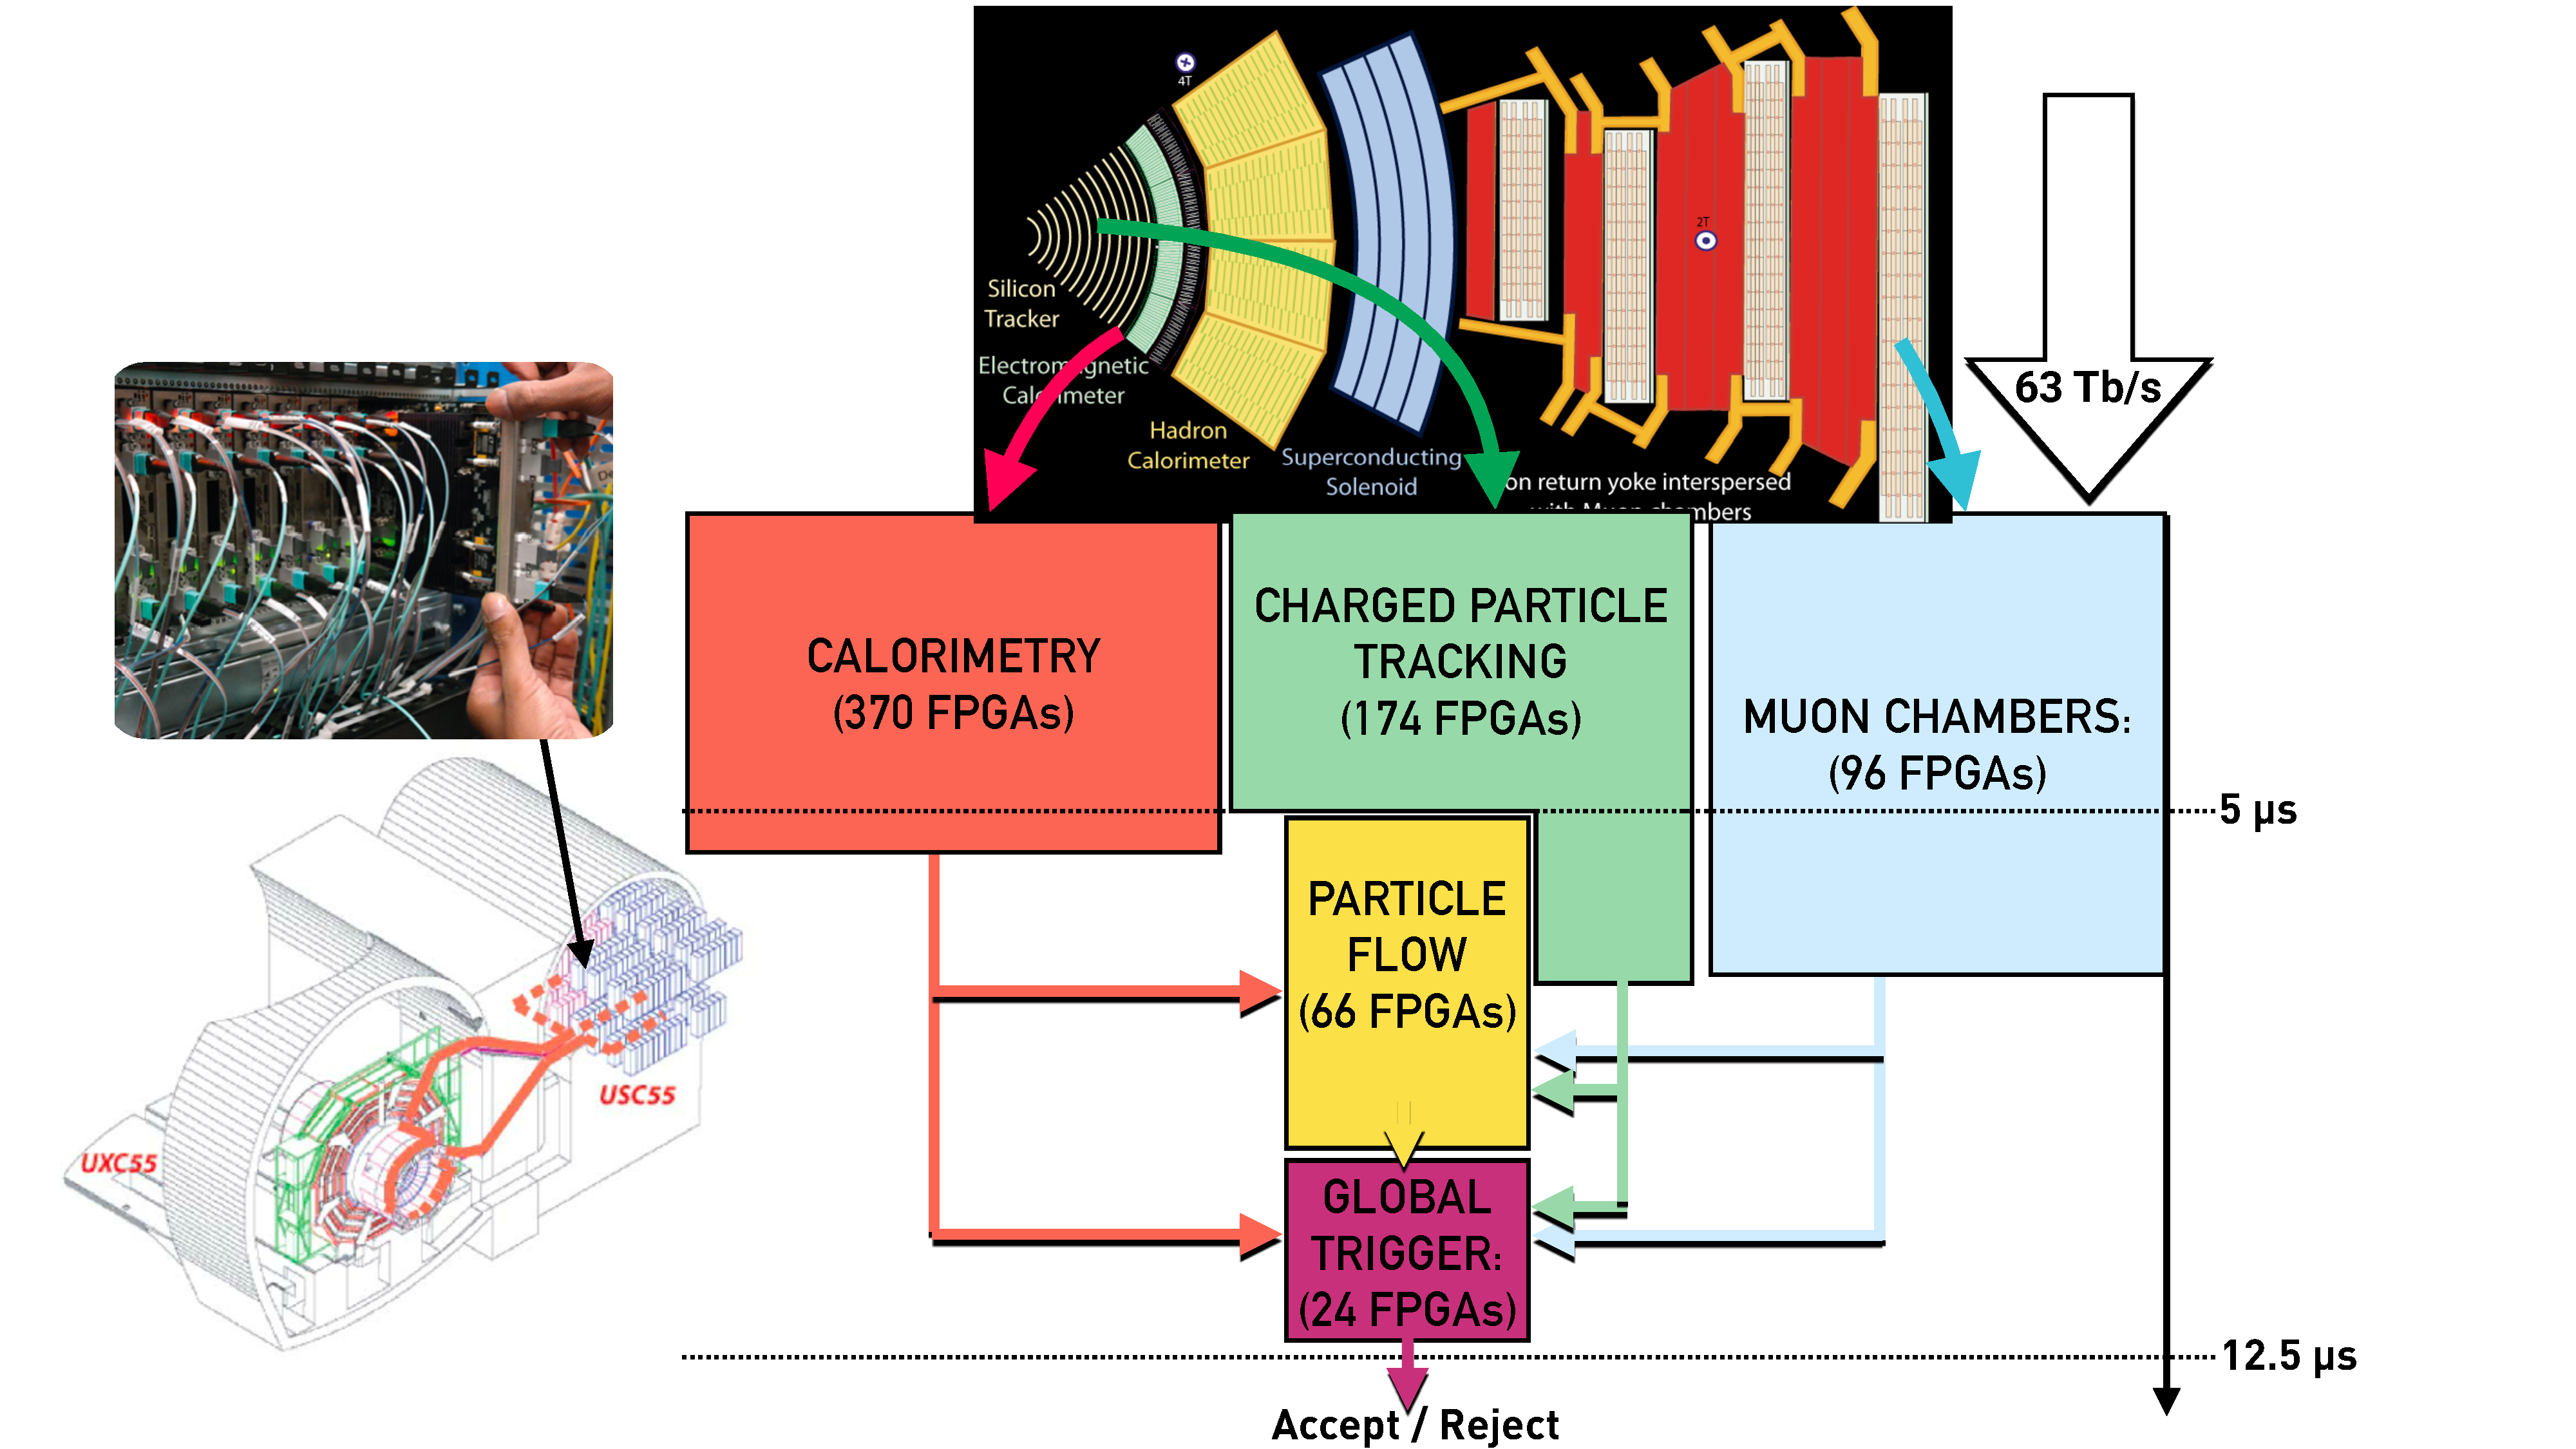
\includegraphics[width=0.69\textwidth]{figures/phase2_l1t.pdf}
    \caption{Diagram of the CMS L1 hardware trigger as foreseen for HL-LHC. The system is located in a radiation shielded cavern right next to the CMS detector and consists of hundreds of FPGAs mounted on custom boards. Each subsystem; calorimeters (orange), tracking detectors (green) and muon chambers (light blue), are first reconstructed locally on  hundreds of FPGAs. This information is then sent forward to a system responsible of correlating the information from all subdetectors using the Particle Flow algorithm (yellow). Finally, the global trigger receives all trigger information for the final decision (pink)~\cite{tdr}.}
    \label{fig:phase2}
\end{figure*}
The Phase-1 Level-1 trigger is designed in a hierarchical way. Information from each subdetector is first processed and reconstructed locally. For instance for the calorimeter, the local reconstruction consists of clustering energy deposits into disentangled showers from individual particles. Local information from each sub system is passed on-wards and combined into particle-level information, using an algorithm called Particle Flow~\cite{Sirunyan_2017}. These features are again combined into higher level objects (like jets, muons, electrons/photons, taus, missing energy) that are passed as input to binary selection algorithms in the Global Trigger. For each local reconstruction of a subsystem, hundreds of FPGAs are used.

\subsection{Machine Learning-based reconstruction}
Recently, significant effort has been made into developing powerful and expressive ML algorithms for fast reconstruction. One example is the demonstration of a graph neural network for clustering of energy deposits in irregular geometry detectors~\cite{garnet}. A second example is a graph neural network based architecture that mimics Particle Flow; combining information from all sub detectors into particles of a given type. A comparison of the reconstruction performance that can be obtained with the classical algorithm versus that which can be obtained with a ML surrogate, is shown in Figure~\ref{fig:mlpf}.
\begin{figure*}[ht]
    \centering
    \includegraphics[width=0.99\textwidth]{figures/mlpf.pdf}
    \caption{The classical Particle Flow reconstruction algorithm (left) versus a graph neural network (right)~\cite{mlpf}.}
    \label{fig:mlpf}
\end{figure*}
These algorithms are currently being explored for offline reconstruction or for the High Level Trigger, but are not yet being developed for Level-1. This requires expertise in deploying models in extremely high throughput and low latency environments, which is where I have experience.

\subsection{AI engines and distributed inference: Accelerating reconstruction}
In order to deploy large models that must cope in extreme throughput/latency conditions, there is a need for dedicated systems and hardware. More and more dedicated AI processors are being developed to accelerate inference of large ML models. One example is the Xilinx Versal AI processors which contain 400 AI processors as well as FPGA fabric, where data can move back and forth between AI Engines and FPGA. There is also significant research being done on distributed inference: where a single ML model can be split over multiple FPGAs and data can move quickly between the different FPGAs. This work is being pioneered by, among others, Gustavo Alonso's group at ETH. 

\subsection{Putting it together: End-to-end}
The ultimate goal is to replace all the intermediate steps of local reconstruction in the Level-1 trigger by a single model or a mixture-of-experts family of models. Powerful large models from Natural Language Processing (e.g. transformer architectures) that could go directly from detector hits to physics objects, approximating the full sequence of local reconstruction and combination, could be deployed on either 1) powerful AI engines or 2) using the existing interconnected FPGAs of the Level-1 trigger design to perform distributed inference. Finding novel, efficient and accurate ways of doing reconstruction during HL-LHC is not a choice, it is a requirement. With the increase in input data size to Level-1 for HL-LHC, our current algorithms for doing reconstruction will be unsustainable.

\subsection{Project components}
In this project we will design and end-to-end ML based flow for hardware event reconstruction in the Level-1 trigger. This most important ingredients are:
\begin{enumerate}
    \item Starting from existing work on offline ML reconstruction for Particle Flow, we will redesign this network for PF reconstruction in the Level-1 trigger. This includes redefining the algorithm to run on Level-1 inputs provided from the subdetectors, and to run distributed over multiple FPGAs to stay within the latency and resource budget of the trigger (also explore hardware solutions).
    \item Extensive validation of this model and testing under varying conditions. Establish and integrate a full flow for data re-training and deployment. Explore online learning/continual learning for adapting the model to changing LHC/CMS conditions. 
    \item After completion of the previous step, we will move one step down in the trigger reconstruction layers and include the local reconstruction in the subdetectors, one subsystem at the time. We begin with distinct ML models that are co-trained (one reconstructing the subdetector information, which then passes its output to the Particle Flow model), then move towards one large model which goes directly from the lowest level information to a particle-output using a foundation model. This could also be the same type of foundation model that will be designed for WP1.
    \item Finally, and after validation of the previous models, we will integrate the reconstruction of final global trigger objects that are used for the trigger decision. 
\end{enumerate}

An illustration of the final AI-powered end-to-end reconstruction design is showed in Figure~\ref{fig:e2e}.

\begin{figure*}[t!]
    \centering
    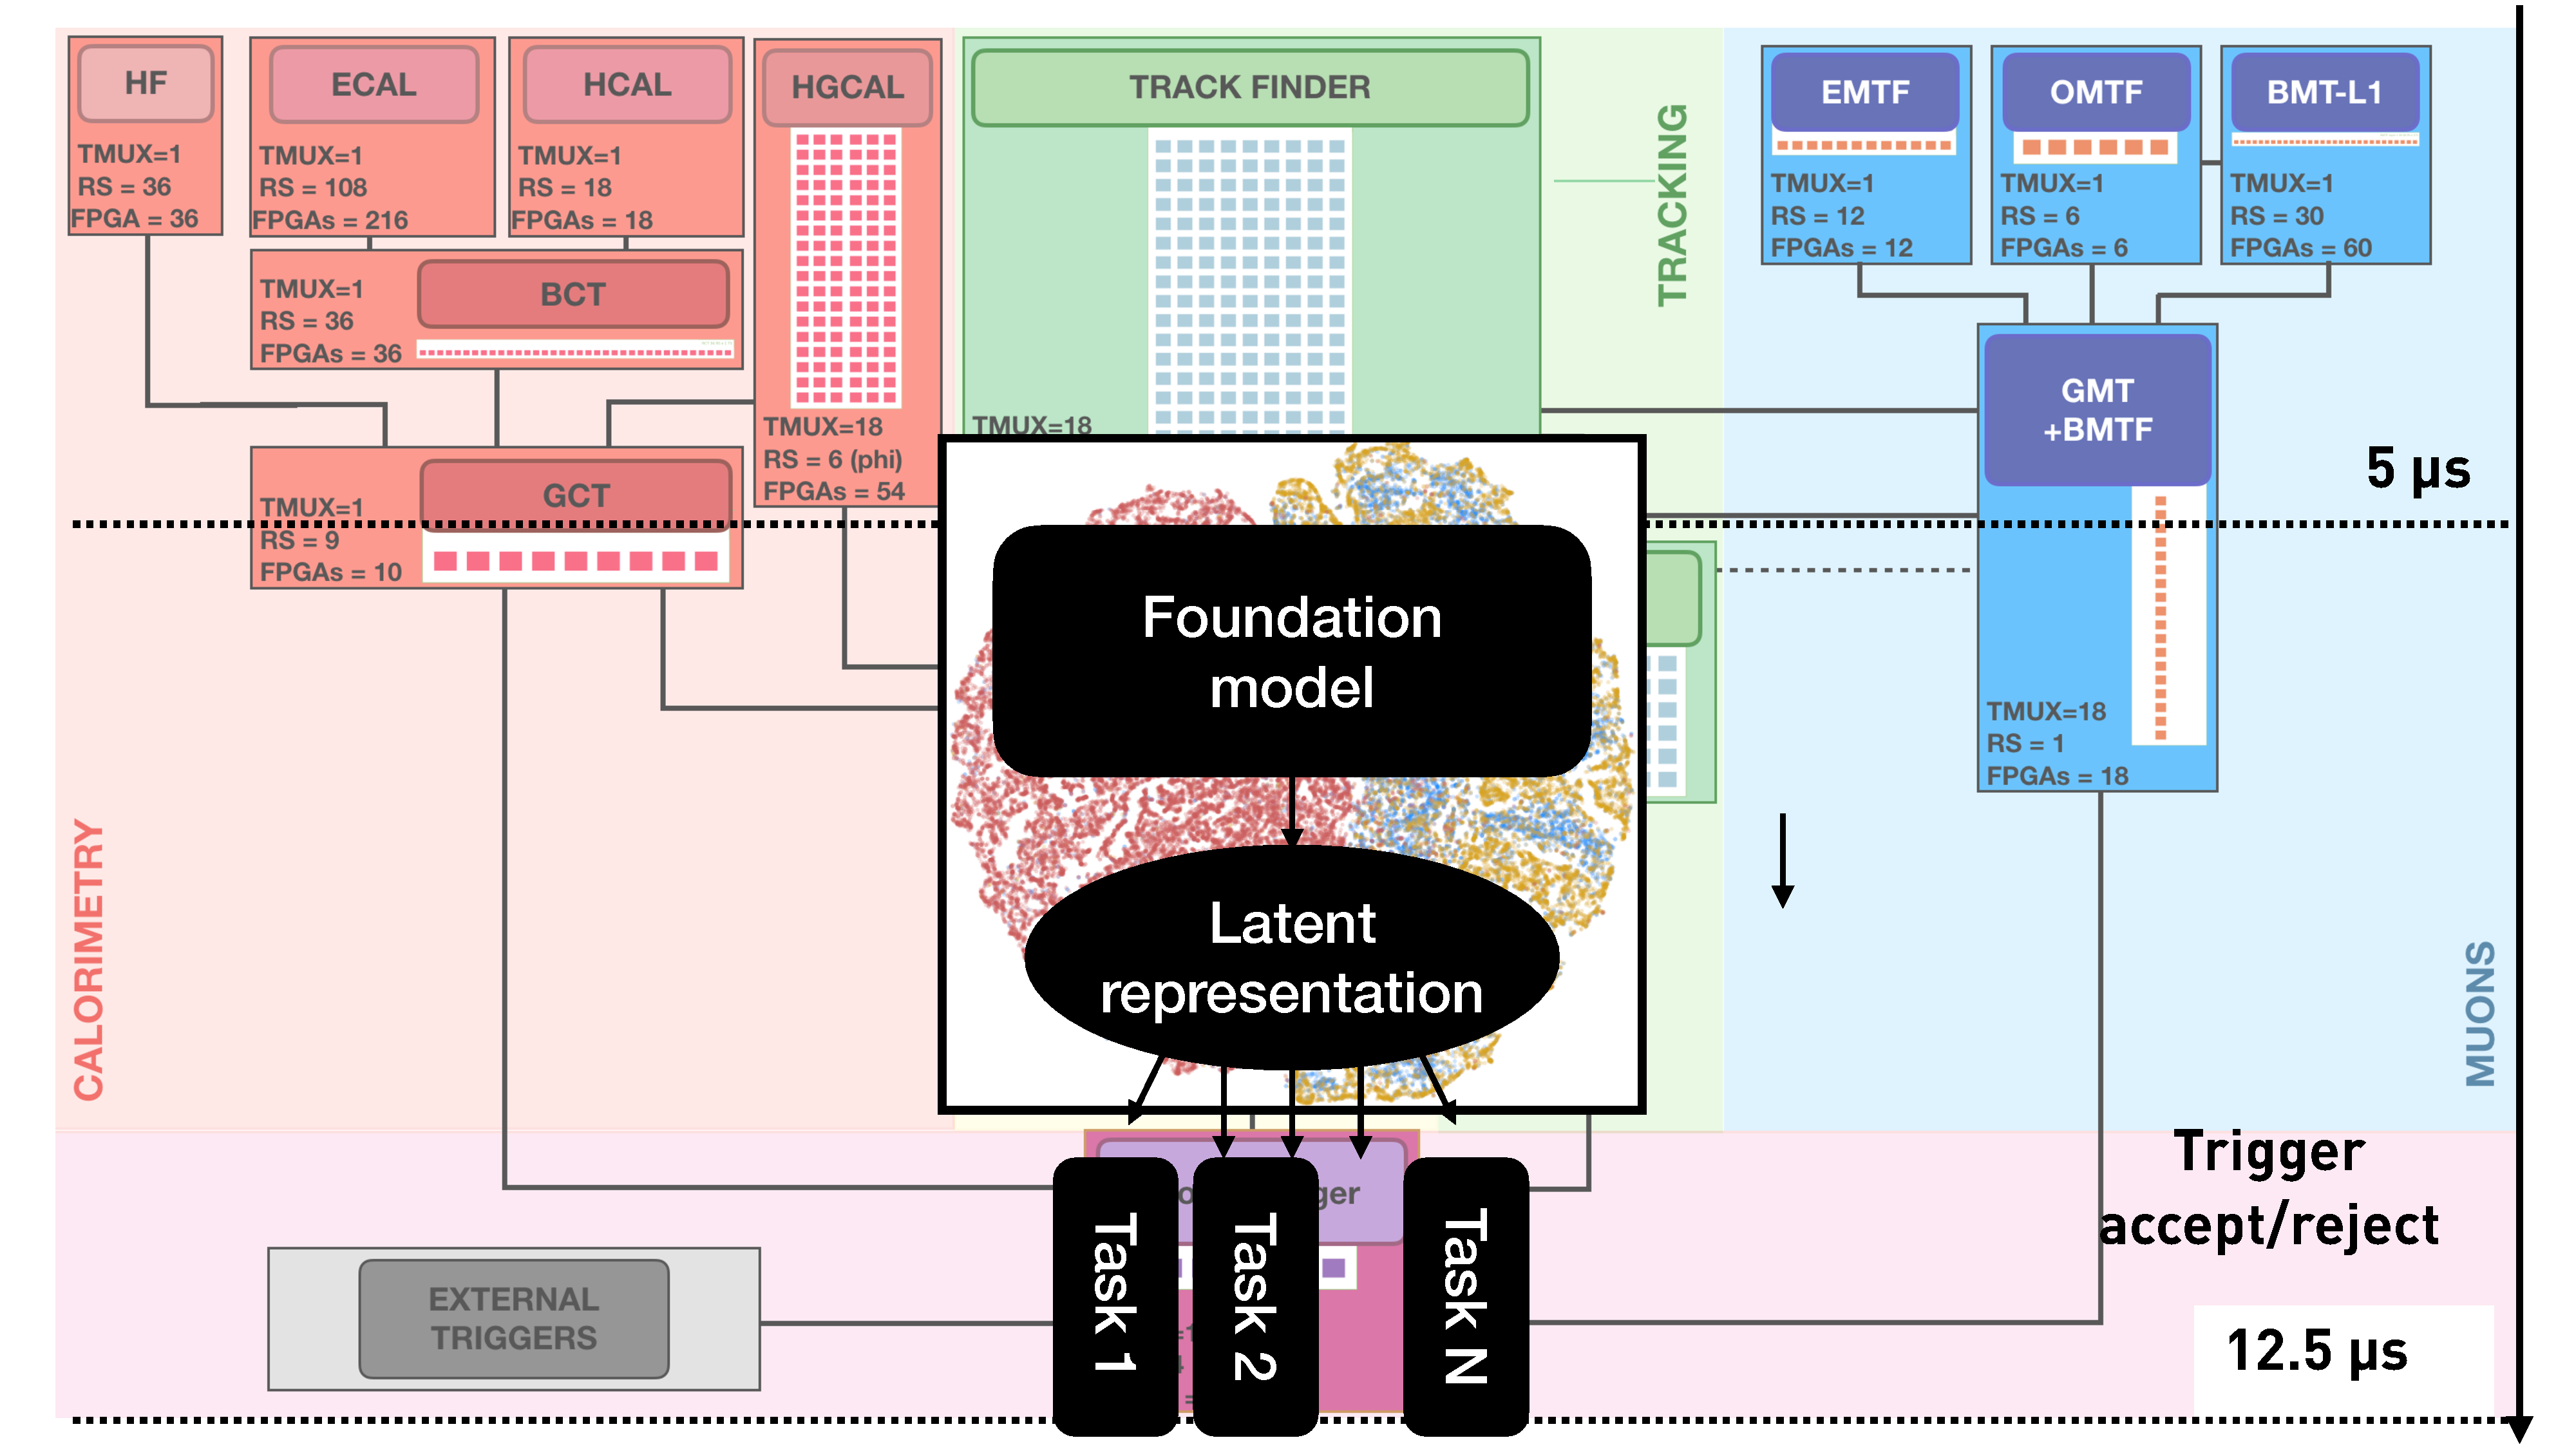
\includegraphics[width=0.99\textwidth]{figures/end_to_end.pdf}
    \caption{The AI-powered end-to-end trigger reconstruction design.}
    \label{fig:e2e}
\end{figure*}


\subsection{WP1: Real-time unbiased New Physics detection with open-world learning}
\subsubsection{Scouting at 40 MHz:}
The 40 MHz scouting system reads out Level-1 trigger data directly from the trigger boards located next to the CMS detector 100 meters under ground. The data is received on dedicated data acquisition boards and sent to the surface at the full bunch crossing rate of 40 MHz. On the surface, buffering capabilities will allow to analyze the Level 1 information for all events at a rate of 40 MHz, but this must be done in semi real-time (depending on the size of the buffer). 
The primary objective is to identify unique physics signatures that are discernible solely from L1 data, yet would evade detection in the Level 1 to High-Level Trigger (HLT) and subsequently to the offline analysis chain. This could for instance be the case for:
\begin{enumerate}
    \item signal processes that have a too large “irreducible” background (e.g. narrow resonances of unknown mass, or
    \item signal processes where signal identification requires an algorithm that can not fit the L1 fixed latency and resource budget (e.g. has too large combinatorics, require too complex reconstruction)
\end{enumerate}

\subsection{Model-independent searches}
 A limiting factor in the search for New Physics is related to how such searches are performed. Searches for new physics processes at particle colliders are usually performed as \textit{blind searches}. Such searches proceed by defining a region of interest in the parameter space, using simulated data of the signal and the Standard Model background processes in order to enhance the data purity. The data is only looked at in the very end where it is tested for the presence of signal through a simultaneous fit of the signal and background probability distributions, hoping to extract a non-zero signal component.

Hundreds of such searches have been performed for hundreds of different potential new particles, but thus far none have been discovered. Despite this, there are still regions of the data that have not yet been probed for the presence of a signal. This has led to an increased interest in more \textit{model-agnostic} search strategies.

ML-based anomaly detection methods have especially been gaining popularity in particle physics as a way of extracting potential new physics signals in a model-agnostic way, by rephrasing the problem as an out-of-distribution detecting task. In this context, model-agnostic refers to assuming no, or at least minimal, prior information regarding the physical model describing the new-physics phenomena. A typical search for new physics signatures involves looking for a specific signal and maximizing the analysis sensitivity for that single model. This analysis is not useful to investigate other new physics models. In an anomaly detection driven search, however, the aim is to be model-agnostic and only look for deviations from the background. This is less sensitive to any model that is biased to a specific signal, yet, it enables the simultaneous search of multiple new physics scenarios. An additional advantage of anomaly detection is that it allows algorithms to undergo direct training on unlabeled data.

\subsection{Novel class detection with Open World Learning}
\begin{figure*}[ht]
    \centering
    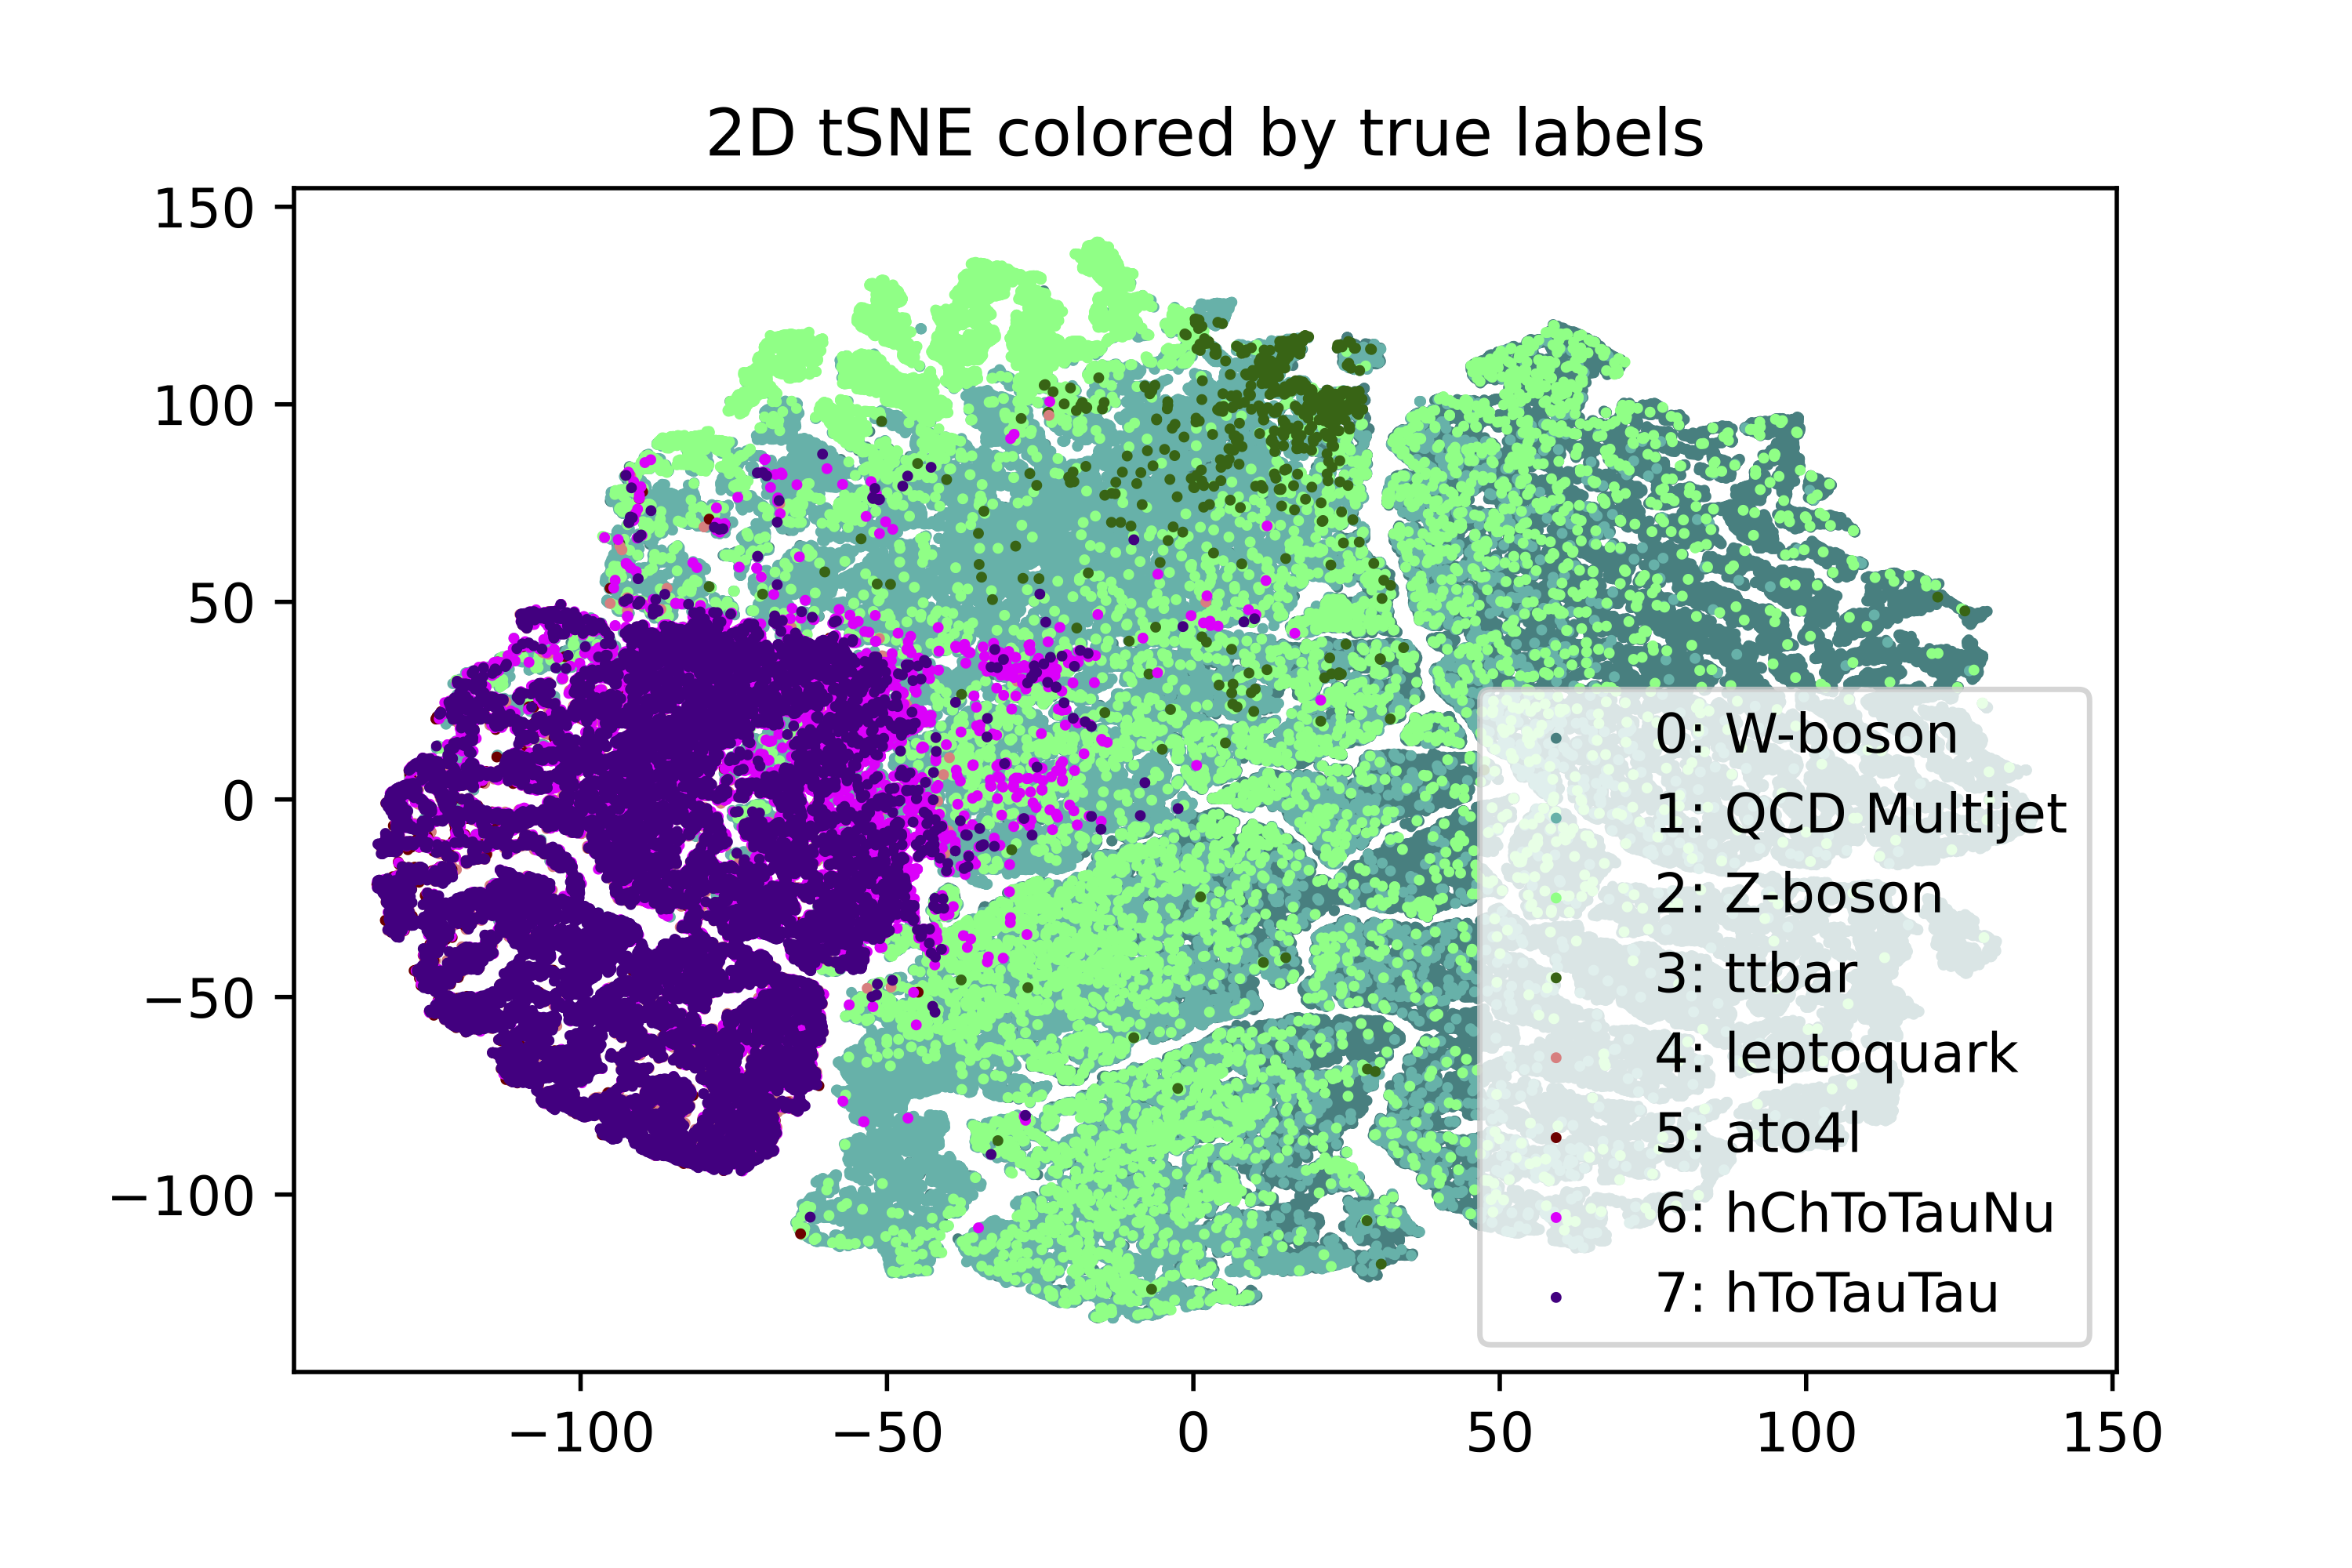
\includegraphics[width=0.49\textwidth]{figures/tSNE_2D_true_labels_10.png}
     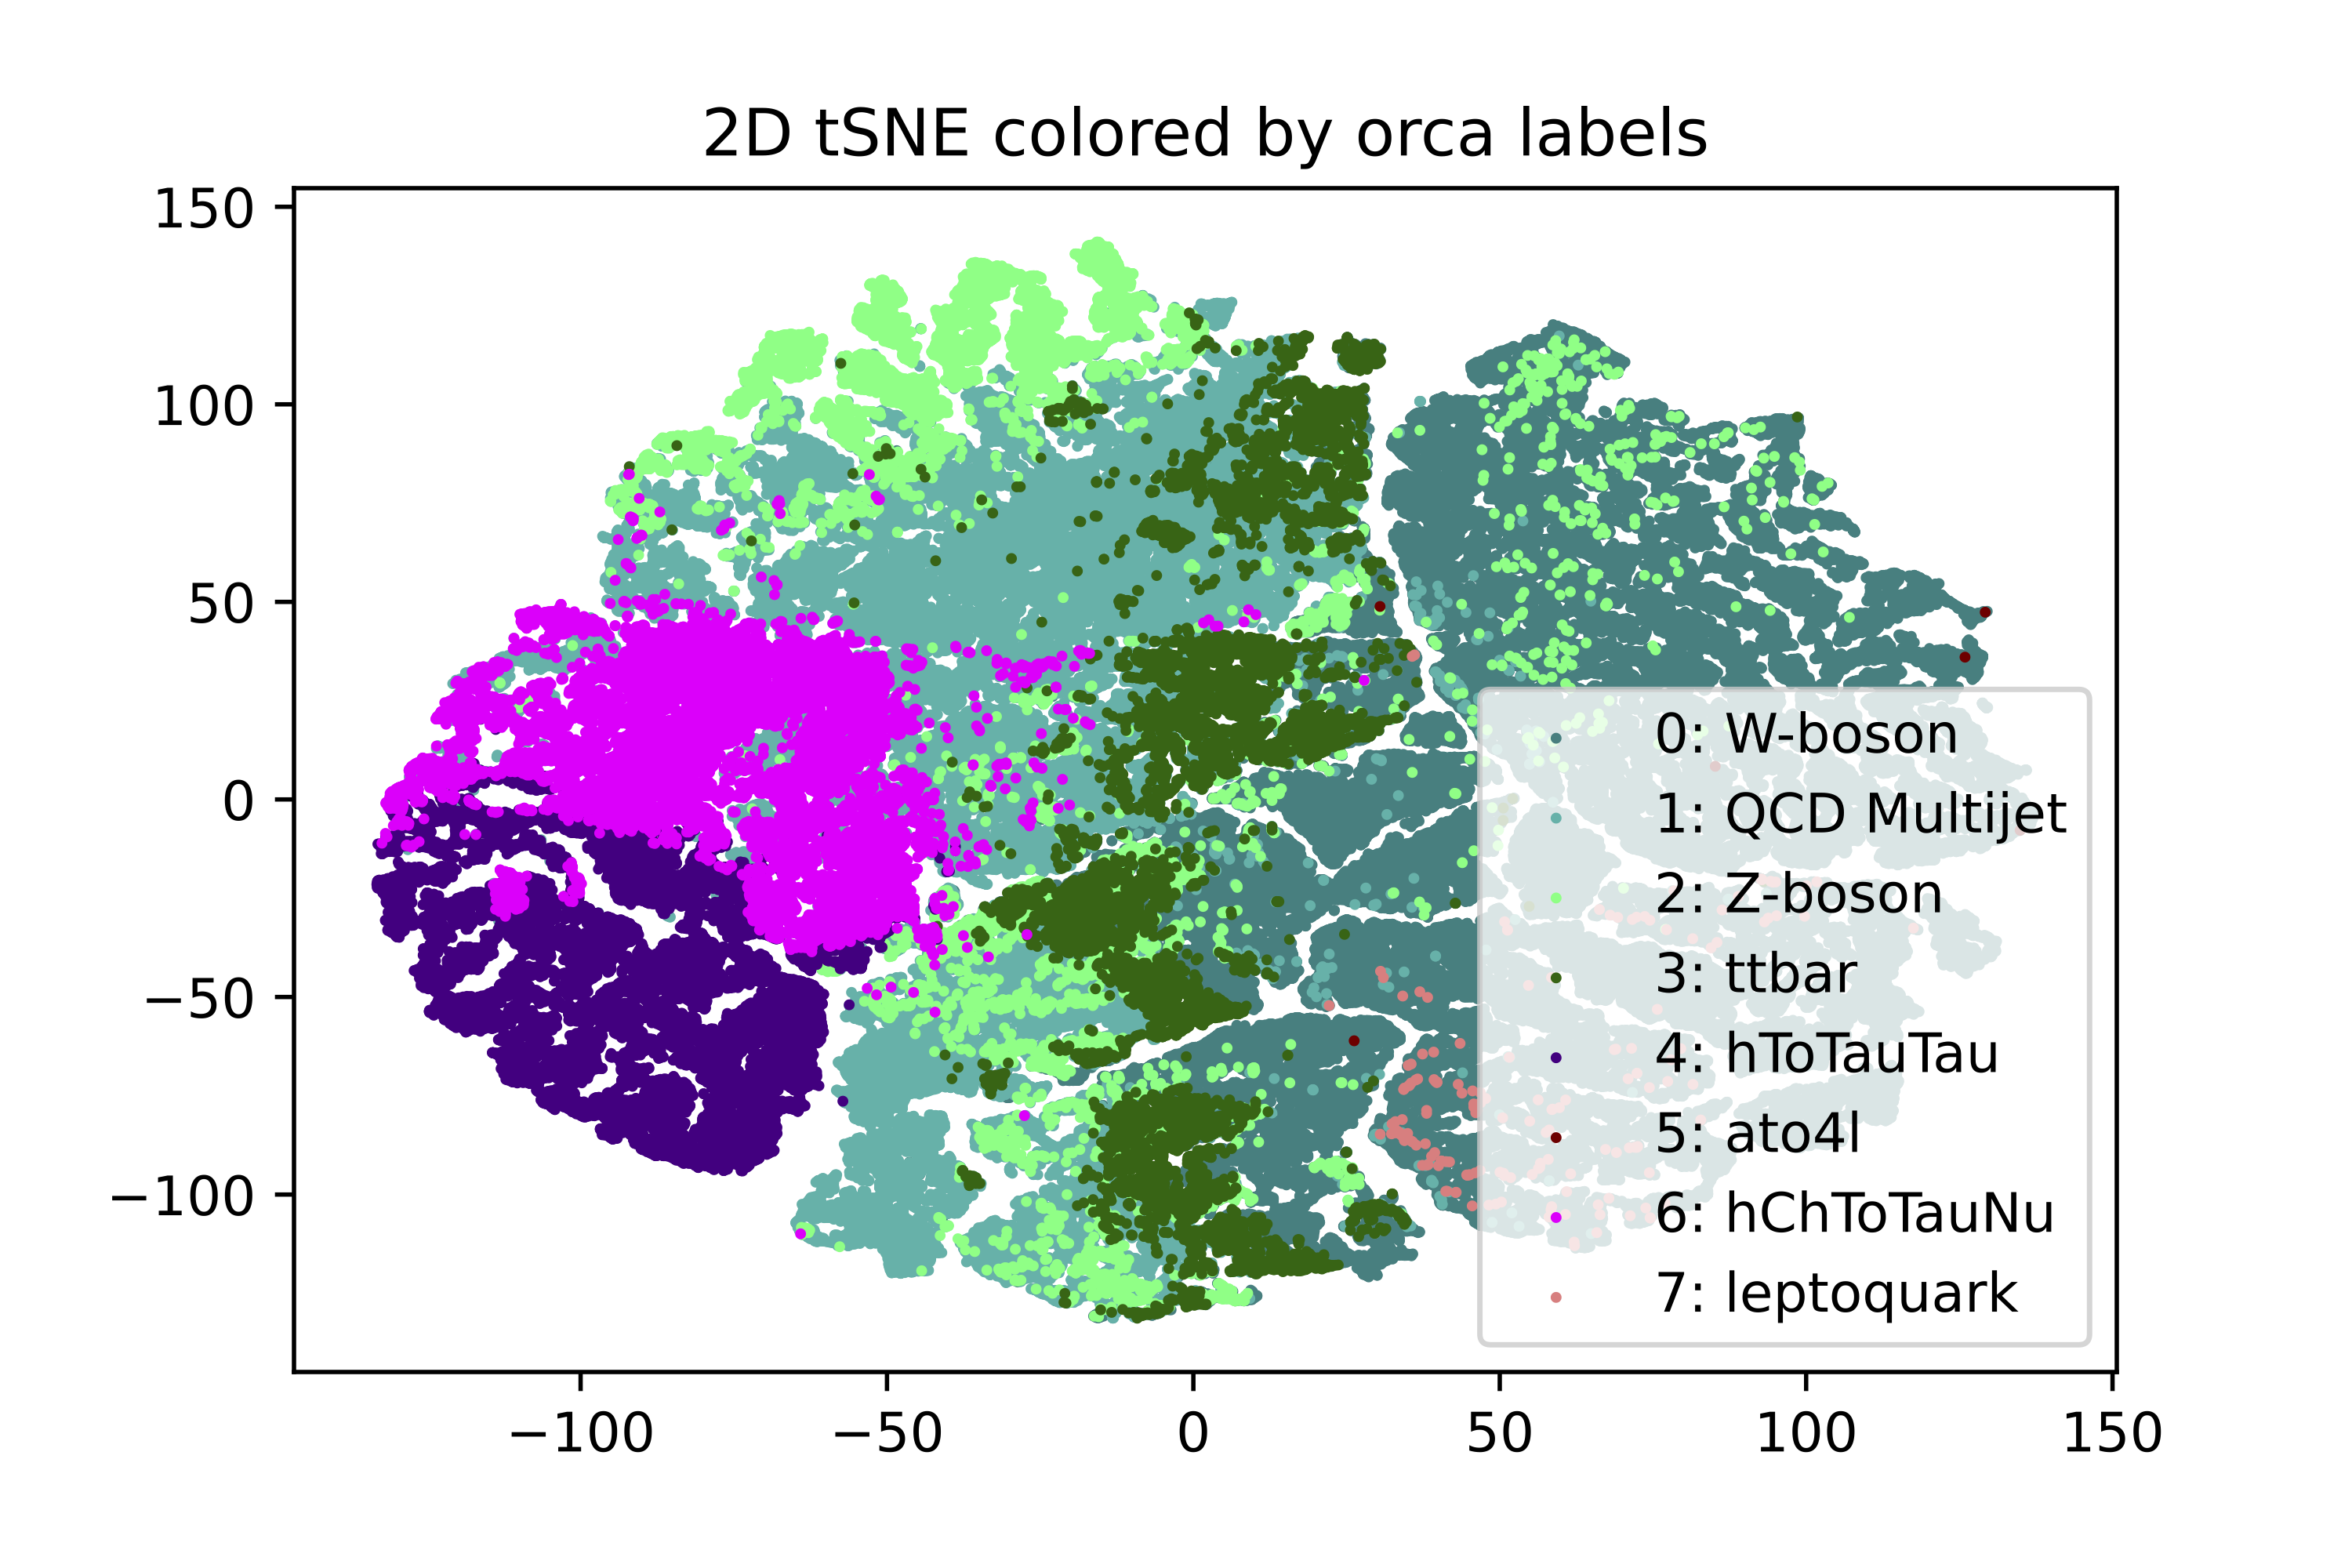
\includegraphics[width=0.49\textwidth]{figures/tSNE_2D_orca_pred_labels_10.png}
    \caption{A t-SNE projection of the embedding space. The colors correspond to the true (left) labels and the predicted labels by ORCA (right). By Kyle Metzger (semester student) }
    \label{fig:orca}
\end{figure*}
Open world learning~\cite{DBLP:journals/corr/abs-2102-03526}, also known as open world recognition, classification, or open-world AI, is becoming crucial as AI agents increasingly interact with real-world environments. Examples include chatbots and self-driving cars, which cannot predict or limit their exposure to only previously encountered scenarios. For instance, a chatbot cannot anticipate every possible user input, nor can a self-driving car assume it has been exposed to all possible real-world scenarios. The essence of open-world AI lies in its ability to recognize the unknown and incorporate this new information, thereby enhancing the AI agent's knowledge base.

Traditional machine learning operates under the closed-world assumption, meaning the classes seen during training are expected to be the same during testing, with no new categories or objects appearing. However, a more realistic approach involves preparing for unseen classes during testing, or open-world scenarios. The objective here is to develop algorithms capable of classifying known data while also identifying and learning from unknown categories. This concept is termed open-world learning or classification. In addition to detecting unseen categories, open-world learning involves the incremental or continual assimilation of these new classes.

Together with a semester student, we have been exploring this way of detecting New Physics as novel classes using the ORCA~\cite{DBLP:journals/corr/abs-2102-03526} paradigm. Assuming we have a range of known classes, which correspond to Standard Model processes, we train an algorithm to identify these classes based on labeled Standard Model Monte Carlo. When we apply this trained algorithm to data, it will itself attempt to assign that new data to a known class (SM) or a novel class (Beyond SM). This workflow is illustrated in Figure~\ref{fig:ow}.
\begin{figure*}[ht!]
    \centering
    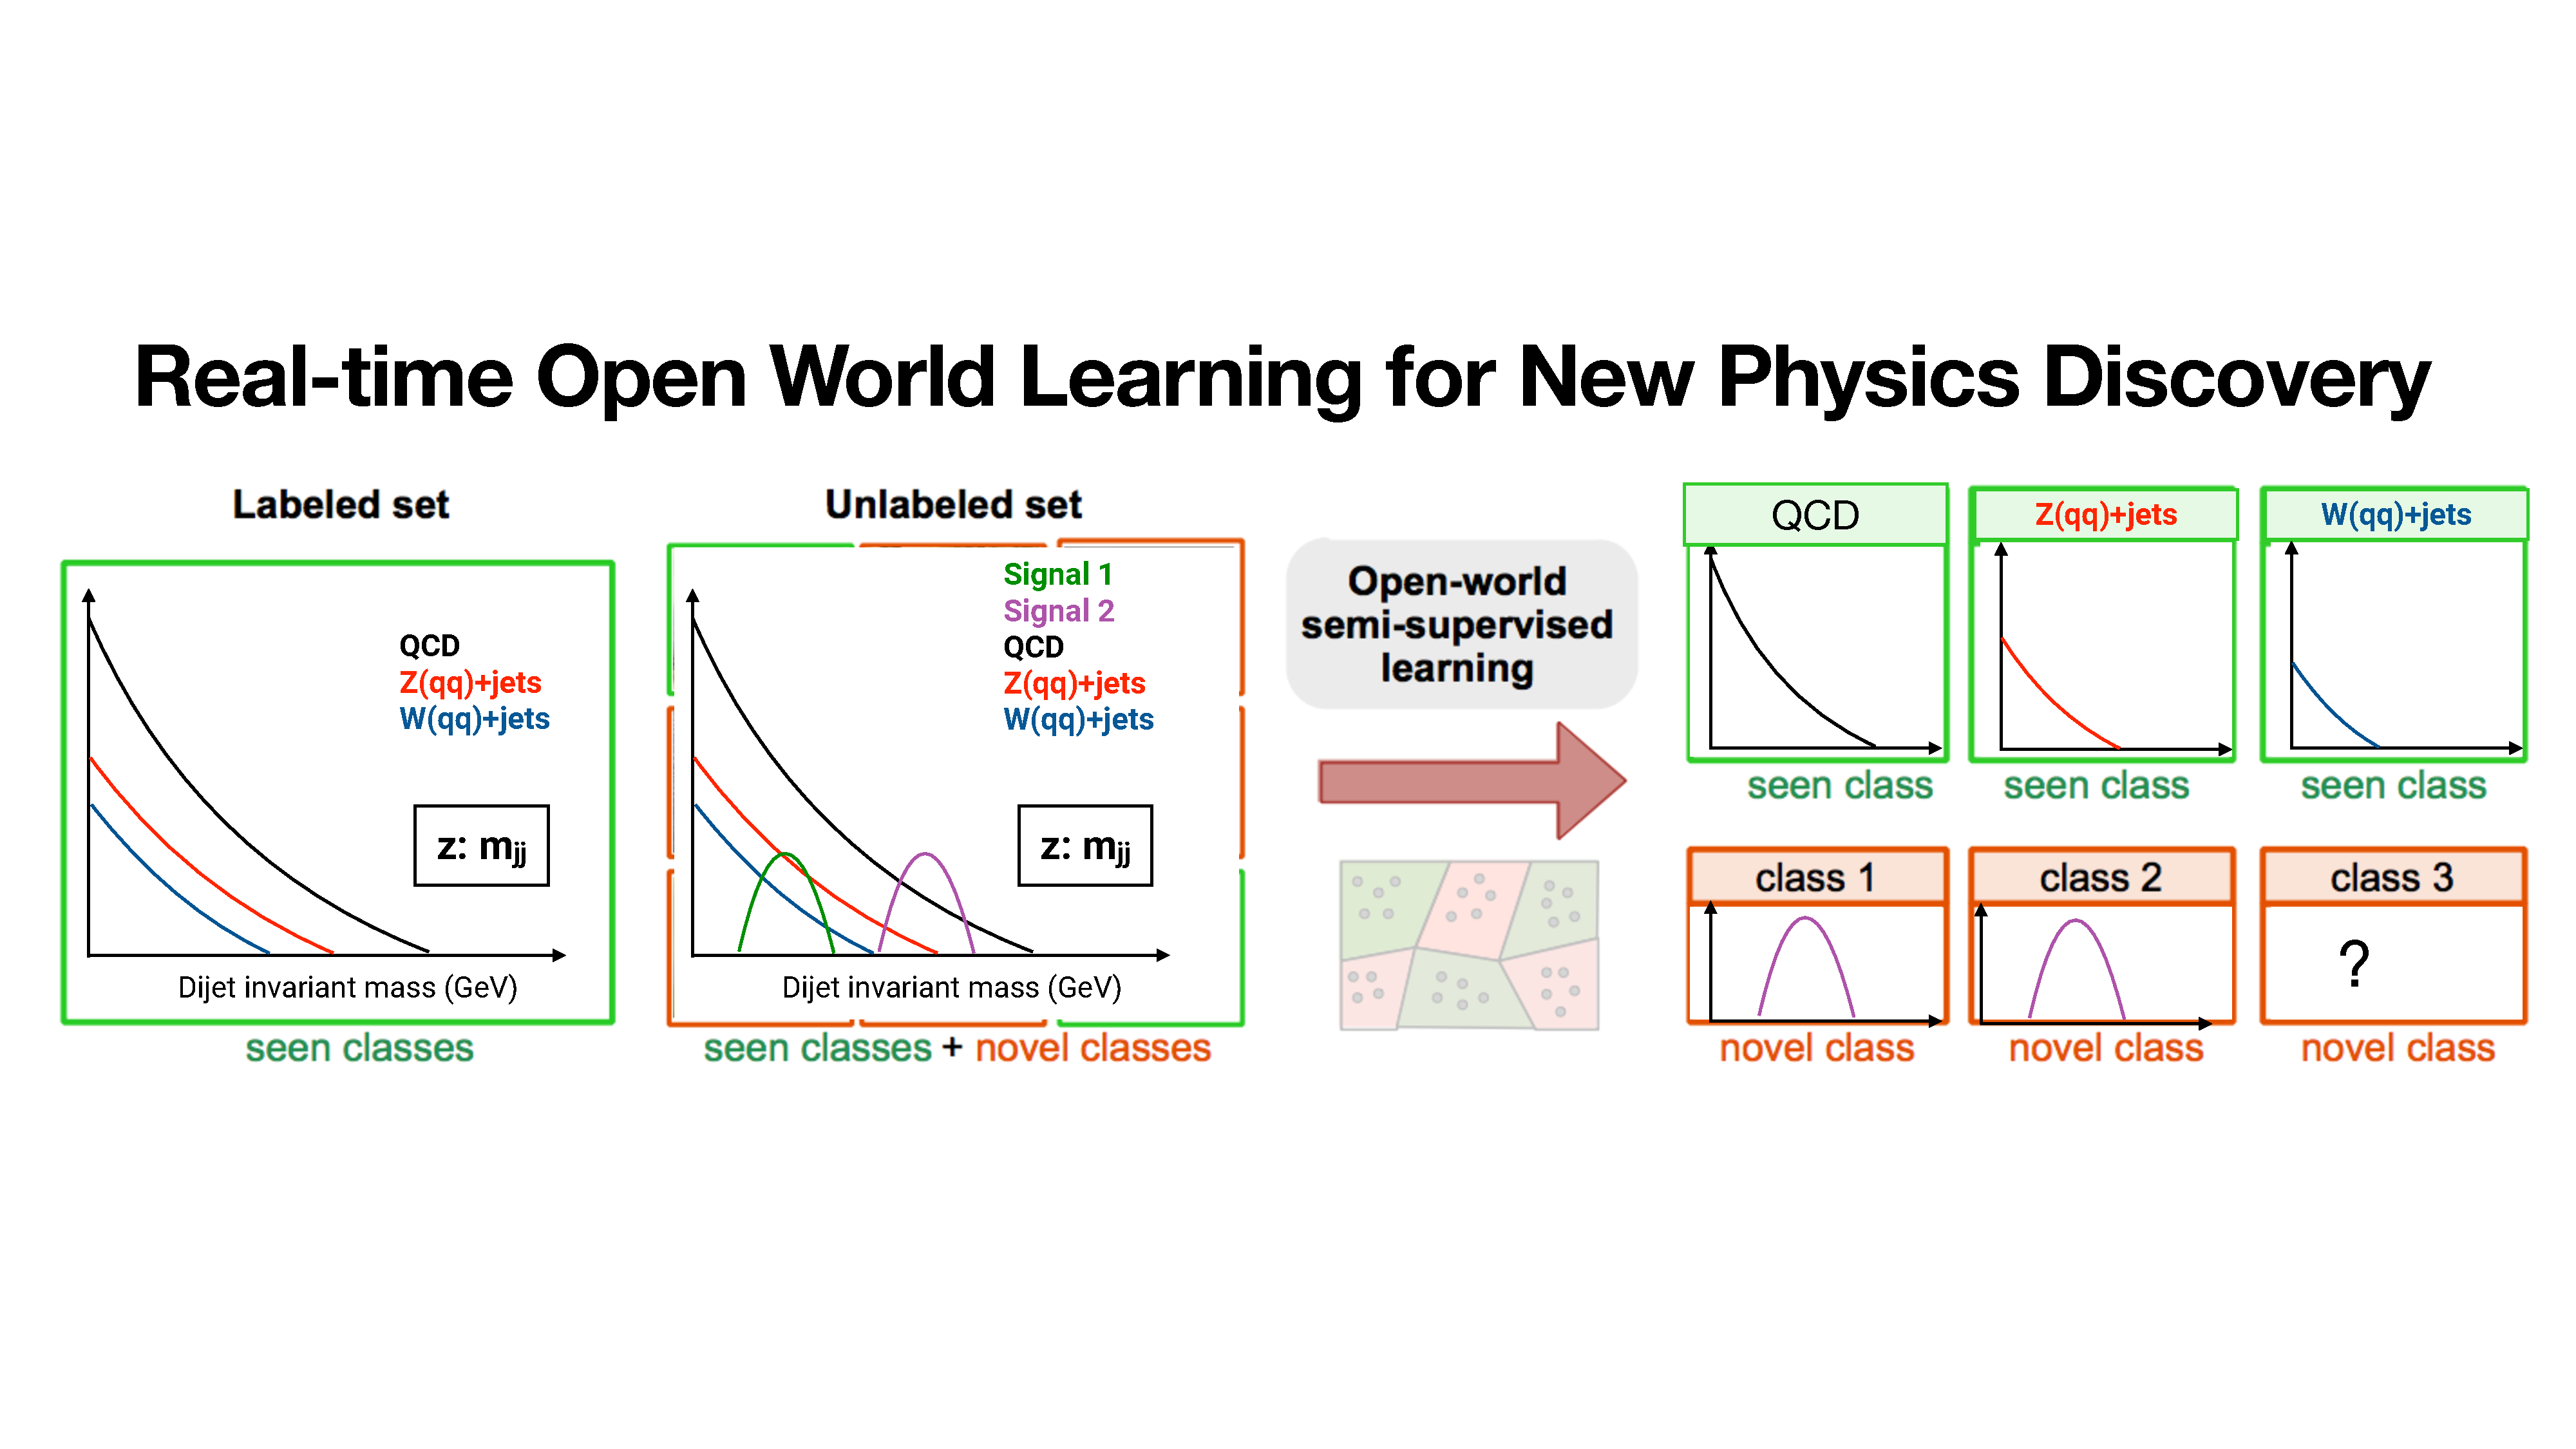
\includegraphics[width=0.99\textwidth]{figures/ow_np.pdf}
    \caption{An illustration of the open-world learning for new physics discover workflow. Starting from a labeled dataset and a powerful data representation, an algorithm is trained to identify novel classes in an unseen dataset}
    \label{fig:ow}
\end{figure*}

An initial result is shown in Figure~\ref{fig:orca}. Training an algorithm on known SM processes only, we attempt to discover novel classes in a never seen before dataset. This dataset mimics the SM processes we would expect to see in CMS, but also has a few novel signals injected that the algorithm has not seen during training. We observe that we are able to accurately identify these novel classes, without having been given explicit information about them.

The initial classifier needs to provide a powerful embedding of particle physics data. For this we will explore \textit{foundation models}. These are models that are trained on a broad set of unlabeled data and which can be used for different tasks, with minimal to no fine-tuning. An example of such a model trained unsupervised to distinguish different type of particles is shown in Figure~\ref{fig:jet}.

\begin{figure*}[ht]
    \centering
    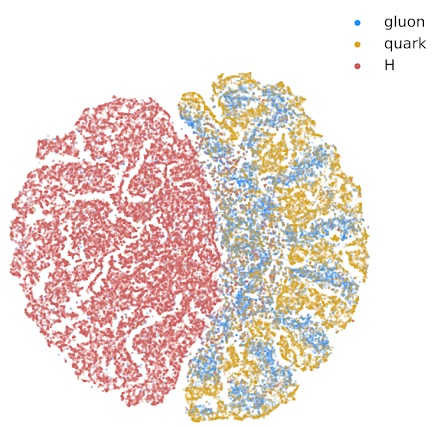
\includegraphics[width=0.49\textwidth]{figures/foundation_cl.jpg}
    \caption{A foundation model trained self-supervised to learn a representation of jets~\cite{foundation}.}
    \label{fig:jet}
\end{figure*}



\subsection{Project components}

In this project we will design an open world novel class detection algorithm that will run in semi real-time in the 40 MHz scouting system. The most important ingredients are:
\begin{enumerate}
    \item The initial classifier needs to be extremely powerful. We will design a backbone/foundation ML model based on SM simulation that incorporates a powerful embedding allowing it to discriminate between various known classes, but also be powerful enough to identify a wide variety of unknown (potential) classes (using techniques like contrastive learning).
    \item We must design the algorithm to run in semi real-time in the scouting online processing and provide summary statistics that are powerful yet contain enough information to let us further understand the properties of potential novel classes that are identified. Storing all of the scouting data would correspond to O(100) Pb/year, so the data must be reduced to something manageable. 
    \item We must design a rigorous interpretability framework. If novel classes are discovered, we need to understand what sets them aside from seen classes using powerful clustering techniques like self-clustering maps~\cite{6790553}.
\end{enumerate}

Running a real-time, model-independent search in the scouting system using modern open world AI is a fundamentally new way to search for New Physics in CMS without theory assumptions or event filtering bias. It would open the door to a wide range of hitherto uncovered New Physics phase-space.

\section{Summary}
\begin{figure*}[bht!]
    \centering
    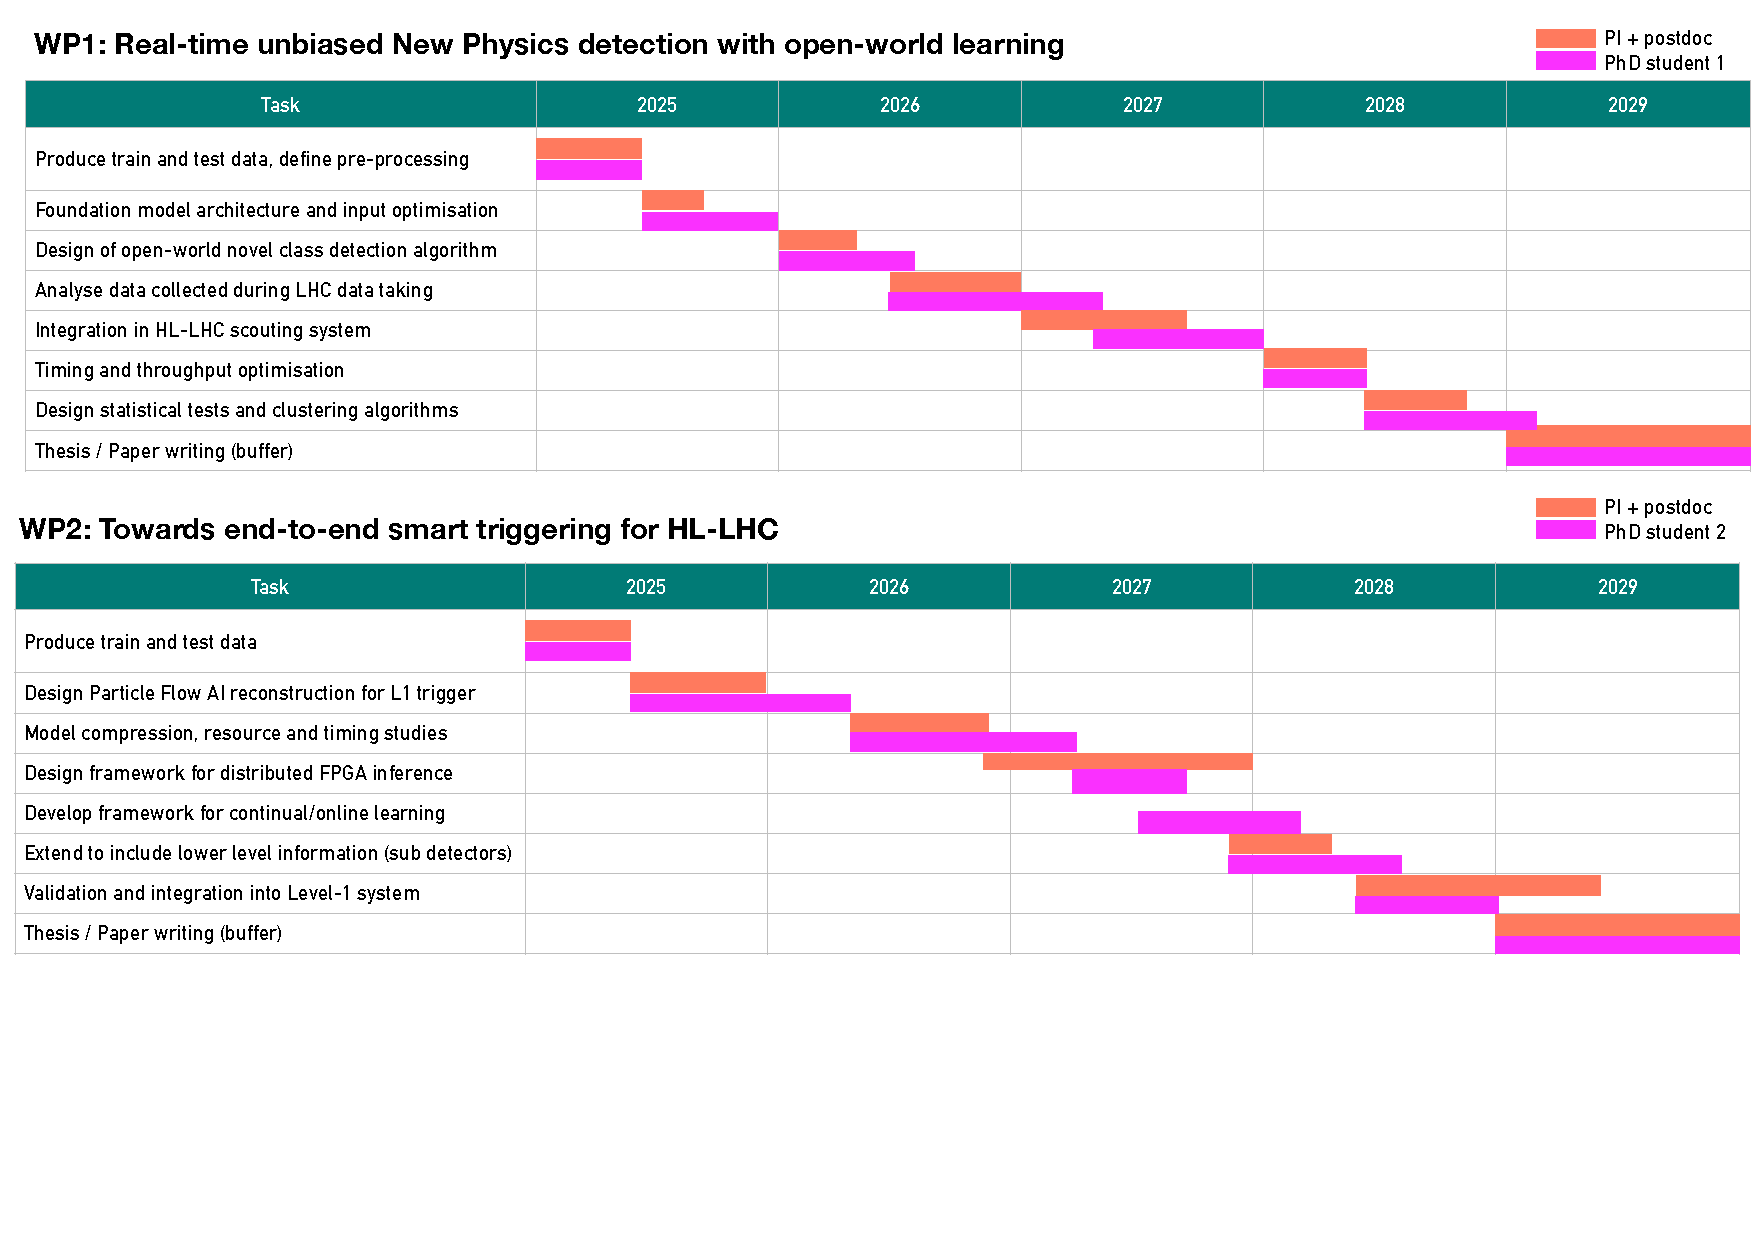
\includegraphics[width=0.99\textwidth]{figures/GanntChart_SG.pdf}
    \caption{A detailed project schedule for the two work packages. The orange line corresponds to the PI and postdoc and the purple to the PhD student.}
    \label{fig:gannt}
\end{figure*}
An overview and timeline over both projects proposed here is shown in Figure~\ref{fig:gannt}.
Both are fundamentally new ways of analyzing and reconstructing data in the Level-1 hardware trigger. As we move towards HL-LHC, both will be crucial in order to make sure we maximize our sensitivity to potential New Physics. They require knowledge across a wide range of topics like Machine Learning, FPGA programming, New Physics searches and efficient inference on specialized hardware. I believe I have the necessary experience within all of these. Besides the projects proposed above, I also wish to continue building our group as a center for fast inference in particle physics in Europe and collaborate with researchers from other scientific domains and industry. As coordinator of the Targeted Systems group at the Accelerated AI Algorithms for Data-Driven Discovery (A3D3) Institute, as well as a coordinator of the Fast Machine Learning for Science Lab, I am one of the key contributors to the field of real-time AI in scientific applications (see CV). Within ETH, I see a great opportunity to build bonds with other departments. I have collaborated with T. Delbrueck the Institute of Neuroinformatics, and have initiated collaborations with the group of L. Benini at the ETH Future Computing Laboratory and G. Alonso at the ETH Computer Systems group. These are projects I wish to continue in the future, and their help will be important in realizing a distributed inference algorithm in the Level-1 trigger. Additionally, I have an ongoing collaboration with Google Zurich on designing low-latency algorithms on FPGAs (see CV), which will continue to be crucial for the design of ML-based algorithms for the CMS Level-1 trigger during HL-LHC. As a member of the core team assisting and training the CMS Collaboration as a whole to perform nanosecond inference in the Level-1 trigger, I believe our group at ETH will play a crucial role for the success of CMS during HL-LHC.

\bibliographystyle{cms_unsrt}
\bibliography{bibliography}

\end{document}

